\documentclass[11pt]{article}

\usepackage[a4paper,margin=25mm]{geometry}
\usepackage[T1]{fontenc}
\usepackage[utf8]{inputenc}
\usepackage{amsthm}
\usepackage{newtxtext,newtxmath}
\usepackage{microtype}
\usepackage{mathtools,bm}
\usepackage{booktabs,array,tabularx,longtable,multirow}
\usepackage{graphicx}
\usepackage[dvipsnames]{xcolor}
\usepackage{enumitem}
\usepackage{csquotes}
\usepackage{fancyhdr}
\usepackage{caption}
\usepackage{subcaption}
\usepackage{url}
\usepackage{siunitx}
\usepackage{hyperref}
\usepackage[nameinlink,noabbrev]{cleveref}
\usepackage[backend=biber,style=authoryear,maxcitenames=2,maxbibnames=99,doi=true,url=true,isbn=false,eprint=true]{biblatex}
\addbibresource{references.bib}

\definecolor{Aubergine}{HTML}{5B2A86}
\definecolor{Petrol}{HTML}{087E8B}
\definecolor{Saffron}{HTML}{D89B00}
\definecolor{Coral}{HTML}{C8553D}
\definecolor{Slate}{HTML}{44546A}
\hypersetup{
  colorlinks=true,
  linkcolor=Aubergine,
  citecolor=Petrol,
  urlcolor=Coral,
  pdfauthor={Anonymous},
  pdftitle={Certified Commitment Horizons in Dynamic Lot Sizing},
  pdfsubject={Exact prefix stability, optimal-face witnesses and one-step calibration of forecast revisions}
}

\setlength{\parindent}{0pt}
\setlength{\parskip}{0.52em}
\setlist{nosep,leftmargin=1.55em}
\captionsetup{font=small,labelfont=bf}
\pagestyle{fancy}
\fancyhf{}
\fancyhead[L]{Certified commitment horizons}
\fancyhead[R]{Preprint v3.0.0}
\fancyfoot[C]{\thepage}
\setlength{\headheight}{14pt}
\emergencystretch=2em
\allowdisplaybreaks

\newtheorem{theorem}{Theorem}[section]
\newtheorem{proposition}[theorem]{Proposition}
\newtheorem{lemma}[theorem]{Lemma}
\newtheorem{corollary}[theorem]{Corollary}
\newtheorem{remark}[theorem]{Remark}
\newtheorem{example}[theorem]{Example}
\theoremstyle{definition}
\newtheorem{definition}[theorem]{Definition}
\newtheorem{problem}[theorem]{Decision problem}

\newcommand{\R}{\mathbb{R}}
\newcommand{\cI}{\mathcal{I}}
\newcommand{\cO}{\mathcal{O}}
\newcommand{\cP}{\mathcal{P}}
\newcommand{\cG}{\mathcal{G}}
\newcommand{\norm}[1]{\left\lVert #1\right\rVert}
\newcommand{\winf}[1]{\left\lVert #1\right\rVert_{\infty,w}}
\newcommand{\pos}[1]{\left(#1\right)_{+}}
\newcommand{\WWR}{\textsc{WW-Prefix-Radius}\ensuremath{_{\infty}}}
\newcommand{\dhat}{\widehat d}
\newcommand{\ellv}{\ell}
\newcommand{\one}{\mathbf{1}}
\newcommand{\rhofr}{\rho^{\mathrm{fr}}}
\newcommand{\rholo}{\rho^{\mathrm{lo}}}
\newcommand{\rhohi}{\rho^{\mathrm{up}}}
\DeclareMathOperator*{\argmin}{arg\,min}
\DeclareMathOperator*{\argmax}{arg\,max}

\title{\vspace{-1.3cm}\textbf{Certified Commitment Horizons in Dynamic Lot Sizing}\\[0.35em]
\large Exact Prefix Stability, Optimal-Face Witnesses and One-Step Forecast Calibration}
\author{Anonymous}
\date{Preprint version 3.0.0 --- 24 August 2026}

\begin{document}
\maketitle

\begin{center}
\small Version DOI: \href{https://doi.org/10.5281/zenodo.22086554}{10.5281/zenodo.22086554}
\end{center}

\begin{center}
\fcolorbox{Petrol}{Petrol!6}{\begin{minipage}{0.93\linewidth}
\textbf{Assurance status.} This candidate release separates the abstract forced-source path model from its classical lot-sizing interpretation. The latter is invoked only under the proved active-horizon bridge: every admissible revision has positive first-period demand support, and every later setup cost is strictly positive. Every value labelled \emph{certified} is computed or re-verified in exact rational arithmetic with zero tolerances; floating-point optimisation proposes candidates but does not decide certification, topology or infinity. The frozen package contains source, tests, raw audit rows, a separately written certificate checker, version-matched provenance, file hashes and a source-specific inspection receipt for Richter--V{\"o}r{\"o}s (1989). It has not received journal peer review, proof-assistant verification, independent clean-room reproduction or prospective field validation.
\end{minipage}}
\end{center}

\begin{abstract}
Repeated forecast revisions can change near-term production setups after an organisation has begun to act. We define the \emph{strong prefix-stability radius}: the weighted, floor-truncated $L_\infty$ distance from a nominal demand forecast to the nearest revision at which some optimal replenishment path can leave a protected setup prefix. The mathematical core is a forced-source Wagner--Whitin path graph. A new semantic-bridge theorem proves that this graph is exactly the classical active-horizon uncapacitated lot-sizing model, at the level of optimal setup schedules, when the first-period demand floor is positive and all later setup costs are strictly positive. Inputs outside that domain remain valid graph instances but are labelled graph-only; this prevents leading-zero demand or costless empty setups from masquerading as operational instability.

Ordered reduced slopes make every path cost affine in demand. We derive an exact floor-aware distance to a tie with a fixed path, a prefix-deviation directed acyclic graph, and a polynomial frozen-comparator lower certificate. The certificate is exact for a complete path and can be strict for a partial prefix. A compact inverse linear programme supplies a certified upper witness, so coincident bounds close the strong radius without enumeration. We then prove three structural results. The longest prefix common to every nominal optimum determines whether the radius is positive. The exact prefix radius is the minimum of at most $k$ one-protected-arc radii on suffix sub-instances. At every finite nearest destabilisation, the optimal face contains a prefix-retaining and a prefix-leaving adjacent path pair; those paths differ on one contiguous divergence--remergence detour. This compresses every boundary witness to a single structural exchange.

Exact escalation remains finite but worst-case exponential in the released enumeration; the demand-induced one-arc complexity classification remains open. A polynomial-size production-balance mixed-integer formulation avoids exponential front-loading while preserving unresolved solver states. One-step split-conformal calibration controls the next forecast revision only under exchangeability, and a deterministic rolling bound prices structural commitment under quantity recourse. Exact finite audits include the semantic bridge, optimal-face edge witnesses, fixed-path certificates, disjunctive closures, compact-model equivalence and rolling cases. An illustrative demand-series exercise uses reconstructed forecast vintages and stylised costs; it demonstrates the interface, not operational benefit. A page-specific negative reading of Richter--V{\"o}r{\"o}s (1989) found fixed-solution scalar-parametric stability but no protected-prefix object; this supports the stated contribution boundary without asserting exhaustive priority.
\end{abstract}

\noindent\textbf{Keywords:} dynamic lot sizing; Wagner--Whitin; nervousness; commitment horizon; stability radius; inverse optimisation; shortest path; conformal calibration; rolling horizon.

\tableofcontents
\clearpage

\section{The decision problem}\label{sec:decision}

A fixed calendar fence answers a scheduling convention, not a robustness question. The relevant decision is instance-specific:

\begin{quote}
How far must the current demand forecast move before an optimal schedule may change any protected setup epoch or replenishment-cycle boundary?
\end{quote}

\paragraph{Semantic contract.}
The graph theorems use a \emph{forced-source path model}: every complete path begins at period $1$, and graph paths remain distinct even when they differ only by a zero-quantity, zero-cost setup node. This is an exact combinatorial model in its own right. We invoke the ordinary classical lot-sizing interpretation only in \emph{classical active-horizon mode}, which requires
\begin{equation}\label{eq:bridgeconditions}
\ell_1>0,
\qquad
K_i>0\quad(i=2,\ldots,T).
\end{equation}
\Cref{thm:semanticbridge} proves that these conditions make the forced source productive for every admissible revision and remove encoding-only ties from empty later setups. Every software record declares one of these two modes. Unless a result is explicitly called a classical corollary, its universal mathematical statement is at graph level.

Periods are $1,\ldots,T$. A complete path
\[
P=(v_0=1<v_1<\cdots<v_m=T+1)
\]
encodes replenishment cycles: arc $(v_r,v_{r+1})$ sets up in period $v_r$ and covers demand through period $v_{r+1}-1$. Fix a nominal forecast $\dhat\in\R_+^T$, a selected nominal optimal path $P^\star$, and its first $k$ arcs
\[
\pi_k=(v_0,\ldots,v_k).
\]
Let
\[
\cI_k=\{P:P\text{ starts with }\pi_k\},
\qquad
\cO_k=\cP\setminus\cI_k,
\]
and define the best prefix-retaining and prefix-leaving costs at revised demand $d$ by
\[
A_k(d)=\min_{P\in\cI_k}C_P(d),
\qquad
B_k(d)=\min_{Q\in\cO_k}C_Q(d).
\]
A tie already permits a rational schedule change. Thus the prefix is compulsory for every optimum exactly when $B_k(d)>A_k(d)$.

Let $w\in\R_{++}^T$, let $\ellv\in\R_+^T$ satisfy $\ellv\le\dhat$, and put
\[
\norm{x}_{\infty,w}=\max_t w_t|x_t|.
\]
Weights set the coordinate scale; they are directionally symmetric. Direction-specific revision penalties would require a genuinely asymmetric gauge and are outside the present results. Floors are declared input semantics, not quantities inferred by the method: a floor may encode empirical or physical demand support, a contractual or planning minimum, or a deliberately conservative truncation. These interpretations produce the same mathematical lower bound but are not operationally interchangeable, and the provenance of an application must identify which is intended.

\begin{definition}[Strong prefix-stability radius]\label{def:radius}
The weighted strong radius of the first $k$ cycles is
\begin{equation}\label{eq:rho}
\rho_{k,w}(\dhat)=
\inf\left\{
\winf{d-\dhat}: d\ge\ellv,\ B_k(d)\le A_k(d)
\right\},
\end{equation}
with the convention $\inf\varnothing=+\infty$. For $w=\one$ we write $\rho_{k,\infty}$.
\end{definition}

The radius freezes structural setup epochs and cycle boundaries. It does not freeze quantities. Under the uncapacitated model, a retained cycle can adjust its order quantity to revised or realised demand.

\begin{problem}[\WWR]\label{prob:decision}
\textbf{Input:} rational $K,q,\dhat,\ellv,w,R$, a declared semantic mode, a nominally optimal path $P^\star$, and $k\in\{1,\ldots,m\}$. Classical active-horizon mode must satisfy \eqref{eq:bridgeconditions}; otherwise the instance is interpreted as a forced-source graph. Nominal optimality may be treated as a promise or checked by one shortest-path calculation.\\
\textbf{Question:} does some $d\ge\ellv$ satisfy
\[
\winf{d-\dhat}\le R
\quad\text{and}\quad
B_k(d)\le A_k(d)?
\]
Equivalently, is $\rho_{k,w}(\dhat)\le R$?
\end{problem}

\begin{proposition}[Basic geometry]\label{prop:geometry}
Assume $P^\star$ is nominally optimal.
\begin{enumerate}[label=(\alph*)]
\item For every $r<\rho_{k,w}(\dhat)$, every optimum at every admissible $d$ with $\winf{d-\dhat}\le r$ retains $\pi_k$.
\item If the radius is finite, a nearest destabilising point exists. At a nearest point, $A_k(d)=B_k(d)$, except that $\rho_{k,w}=0$ may already be a nominal tie; even then $A_k(\dhat)=B_k(\dhat)$.
\item $\rho_{k+1,w}(\dhat)\le\rho_{k,w}(\dhat)$ whenever both prefixes exist.
\item The value depends only on the node prefix $\pi_k$, not on which nominal optimum containing that prefix supplied it.
\end{enumerate}
\end{proposition}

\begin{proof}
Part (a) is the complement of the event in \eqref{eq:rho}. For (b), intersect the admissible domain with a closed ball whose radius exceeds the infimum. This set is compact. Both $A_k$ and $B_k$ are minima of finitely many affine functions and hence continuous, so a convergent destabilising sequence attains the infimum. If $B_k<A_k$ at a nearest point, continuity along the segment from $\dhat$ gives an earlier equality. For (c), $\cI_{k+1}\subseteq\cI_k$ and $\cO_{k+1}\supseteq\cO_k$. Part (d) follows because these two path classes are determined by $\pi_k$ alone.
\end{proof}

\section{Reduced cumulative-demand arcs}\label{sec:reduction}

Let $K_i\ge0$ be setup cost, $p_i$ unit production or purchase cost, and $h_i\ge0$ the cost of carrying one unit from $i$ to $i+1$. Demand is met without backlogging. Under the Wagner--Whitin no-speculative-motive condition
\begin{equation}\label{eq:wwcondition}
p_i+h_i\ge p_{i+1}\qquad(i=1,\ldots,T-1),
\end{equation}
an optimal plan has the zero-inventory-ordering structure used by the shortest-path model \parencite{WagnerWhitin1958}.

Define
\[
H_i=\sum_{s=1}^{i-1}h_s,
\qquad q_i=p_i-H_i,
\qquad D_1=0,
\qquad D_j=\sum_{t=1}^{j-1}d_t.
\]
Condition \eqref{eq:wwcondition} is equivalent to
\begin{equation}\label{eq:orderedq}
q_1\ge q_2\ge\cdots\ge q_T.
\end{equation}

\begin{proposition}[Reduced arc form]\label{prop:reduction}
The physical cost of arc $(i,j)$ equals
\begin{equation}\label{eq:reducedarc}
\bar c_{ij}(d)+\sum_{t=i}^{j-1}H_td_t,
\qquad
\bar c_{ij}(d)=K_i+q_i(D_j-D_i)
=K_i+q_i\sum_{t=i}^{j-1}d_t.
\end{equation}
Summed along any complete path, the local carrying terms assemble the path-independent quantity $\sum_{t=1}^TH_td_t$. Therefore reduced and physical costs have the same optimal paths and the same path-to-path regret.
\end{proposition}

\begin{proof}
For $t\ge i$, the physical unit cost of serving period $t$ from setup period $i$ is
$p_i+\sum_{s=i}^{t-1}h_s=q_i+H_t$, so the arc's physical cost is $\bar c_{ij}(d)$ plus its local term $\sum_{t=i}^{j-1}H_td_t$. Every complete path assigns period $t$ to exactly one cycle, so $H_td_t$ appears exactly once in the path total independently of the path.
\end{proof}

\begin{theorem}[Classical active-horizon bridge]\label{thm:semanticbridge}
Assume zero initial inventory, no backlogging, the ordered slopes \eqref{eq:orderedq}, and the bridge conditions \eqref{eq:bridgeconditions}. For every admissible $d\ge\ellv$:
\begin{enumerate}[label=(\alph*)]
\item every feasible physical plan must open a productive setup in period $1$;
\item no optimal setup pattern contains a later open setup whose cycle serves zero demand;
\item optimal physical setup patterns and optimal complete paths are in cost-preserving bijection, after removal of the path-independent carrying term in \cref{prop:reduction}.
\end{enumerate}
Consequently, the graph quantities $A_k(d)$, $B_k(d)$ and $\rho_{k,w}(\dhat)$ are exactly the corresponding classical setup-schedule quantities in active-horizon mode.
\end{theorem}

\begin{proof}
Because $d_1\ge\ell_1>0$, zero initial inventory and no backlogging force positive production, and hence an open setup, in period $1$. Fix any set of open setups. Assign each unit of period-$t$ demand to the latest open setup no later than $t$. Since $q_1\ge\cdots\ge q_T$, this reassignment cannot increase reduced variable cost and preserves feasibility. It therefore yields the zero-inventory path whose nodes are the open setup periods. If a later setup $i$ serves no demand before the next open setup, deleting $i$ changes no assignment or variable cost and reduces setup cost by $K_i>0$; such a node cannot occur in an optimum. Conversely, every complete path defines a feasible physical plan by producing each cycle's demand at its tail. The two constructions preserve the setup pattern and reduced cost, and \cref{prop:reduction} adds the same carrying term to every path.
\end{proof}

\begin{remark}[What the bridge excludes]\label{rem:bridgeexclusions}
If $d_1$ may be zero, the ordinary model can wait for its first productive setup, whereas the forced-source graph still pays $K_1$. For example, $K=(100,1)$, $q=(1,0)$ and $d=(0,1)$ have graph optimum $101$ but ordinary physical optimum $1$. If a later $K_i=0$, inserting an empty setup can create a distinct co-optimal graph path without changing an operational schedule. Such instances remain admissible in forced-source graph mode, where those semantics are explicit; they are rejected by classical active-horizon mode.
\end{remark}

\begin{table}[t]
\centering
\caption{Dependency and interpretation of the main results.}
\label{tab:dependencies}
\small
\begin{tabularx}{\linewidth}{@{}p{0.29\linewidth}p{0.23\linewidth}X@{}}
\toprule
Result layer & Formal domain & Interpretation ceiling \\
\midrule
Affine paths, tie distance, prefix graph, frozen certificate, exact bracket, disjunction, local decomposition and edge witness & Forced-source directed acyclic graph & Exact combinatorial statements for the declared graph semantics \\
Classical active-horizon corollary & Graph layer plus \eqref{eq:bridgeconditions} & Optimal setup epochs and replenishment-cycle boundaries in the ordinary uncapacitated Wagner--Whitin model \\
One-step calibration & Deterministic radius plus exchangeable revision scores & Marginal coverage for the next forecast revision only \\
Rolling loss bound & Retained setup structure plus uncapacitated quantity recourse & Deterministic structural-cost bound; no service or capacity guarantee \\
\bottomrule
\end{tabularx}
\end{table}

\begin{proposition}[Monge arcs]\label{prop:monge}
For $i<i'<j<j'$ and non-negative demand,
\[
\bar c_{ij}(d)+\bar c_{i'j'}(d)
\le
\bar c_{ij'}(d)+\bar c_{i'j}(d).
\]
\end{proposition}

\begin{proof}
The left side minus the right side is $(q_{i'}-q_i)(D_{j'}-D_j)\le0$.
\end{proof}

For every path $P$, let $i_P(t)$ be the setup period whose cycle contains $t$. Then
\begin{equation}\label{eq:affinepath}
C_P(d)=\kappa_P+\beta_P^\top d,
\qquad
\kappa_P=\sum_{i\in P\setminus\{T+1\}}K_i,
\qquad
\beta_{P,t}=q_{i_P(t)}.
\end{equation}
Ordered slopes provide the first proof attack: they create additive affine geometry and the exact coefficient diameter used in \cref{sec:rolling}. They do not collapse the exact prefix problem to one shortest path, because the minimiser of the inside envelope $A_k$ can switch before an outside path wins.

\begin{proposition}[Membership in NP]\label{prop:np}
The rational decision problem \WWR{} belongs to NP: a yes-instance with
input encoding length $L$ has a certificate of length
$\operatorname{poly}(L)$ verifiable in $\operatorname{poly}(L)$ exact
rational arithmetic.
\end{proposition}

\begin{proof}
A yes-certificate is a pair $(Q,d)$: an outside path (at most $T+1$ node
labels) and a rational revised demand vector. The verifier checks, in
exact rational arithmetic, that $Q$ is a complete path not retaining
$\pi_k$; that $d\ge\ellv$ and $w_t\lvert d_t-\dhat_t\rvert\le R$ for
every $t$; and that $C_Q(d)\le C_{\pi_k}(d)+V_{s}(d)=A_k(d)$, computing
$V_s(d)$ by the $O(T^2)$ suffix recursion. Every intermediate value is a
sum of at most $T+1$ products of input rationals with $d$-coordinates, so
all numerators and denominators stay within $\operatorname{poly}(L)$ bits
and the verification runs in polynomial time; no potentials need be
supplied, since the verifier recomputes the inside envelope itself.

For the certificate-size bound, fix any $Q\in\cO_k$ witnessing the event.
The feasible set
$\{(d,u):d\ge\ellv,\ \winf{d-\dhat}\le R,\ u_s=0,\
u_j-u_i\le\bar c_{ij}(d)\ (s\le i<j\le T+1),\
C_Q(d)\le C_{\pi_k}(d)+u_{T+1}\}$
is a rational polyhedron with $O(T^2)$ rows whose coefficients are input
data, and it is non-empty exactly when $d$ can be chosen destabilising
for $Q$ (\cref{thm:fixedlp}): the potentials can always be raised to
$u_{T+1}=V_s(d)$. A non-empty rational polyhedron contains a point of
encoding length polynomial in the facet encoding length --- a basic
feasible solution whose entries are quotients of subdeterminants of the
constraint data \parencite[Cor.~10.2]{Schrijver1986} --- and projecting
it to $d$ gives the required $\operatorname{poly}(L)$-bit witness. If
nominal optimality of $P^\star$ is not promised, the verifier first
checks it by one exact shortest path. The release ships this verifier as
an executable function, exercised against certified witnesses and
corrupted certificates in the test suite.
\end{proof}

No hardness result or unrestricted polynomial exact algorithm is claimed.

\section{Corpus boundary and contribution boundary}\label{sec:literature}

Classical planning-horizon work asks how much future information is needed before early decisions stabilise \parencite{EppenEtAl1969,LundinMorton1975,LeeDenardo1986,BesSethi1988,ChandSethi1990,FedergruenTzur1994,FedergruenTzur1995,DawandeEtAl2006,DawandeEtAl2007}. Robust and stochastic lot-sizing work instead chooses plans under uncertainty in costs, demand evolution or lead times \parencite{HanafizadehEtAl2019,ForelGrunow2023,WeijersEtAl2025,GuillaumeEtAl2026,LiRomeroMorales2017}. Those models optimise against an uncertainty description or forecast process. The present object conditions on one current finite forecast and asks the inverse local question: the demand-space distance to loss of compulsory-prefix optimality.

Interval-demand minimax-regret uncapacitated lot sizing is a closer algorithmic comparator. \Textcite{Zhang2011} gives a polynomial dynamic programme for a two-stage model, and \textcite{LiRomeroMorales2013} give an $O(T^5)$ algorithm when demand alone is uncertain. Their decision order is
\[
  \min_y\;\max_{d\in\mathcal U}
  \bigl(F(y,d)-F^\star(d)\bigr):
\]
one setup vector $y$ is selected before the interval-demand scenario, then evaluated by worst-case regret against a fully adaptive optimum. \WWR{} instead varies the radius of the uncertainty box and asks whether there exists a nearest scenario at which the two \emph{adaptive restricted envelopes} cross, $B_k(d)\le A_k(d)$. It therefore has different quantifiers, a protected optimal face rather than one fixed first-stage vector, and an inverse nearest-boundary objective rather than minimax regret. The polynomial minimax-regret algorithms do not by themselves classify \WWR{}, but any eventual complexity proof must account for their regeneration-interval dynamic programmes.

The contribution boundary rests on a targeted search frozen on 18 August 2026, not on an exhaustive systematic review. Full text was inspected for \textcite{VanHoeselWagelmans1993}, the working-paper version of \textcite{ChakravartiWagelmans1998}, \textcite{WeijersEtAl2025}, \textcite{LiRomeroMorales2013}, \textcite{EgriEtAl2014}, and a seven-page print scan of \textcite{RichterVoros1989}. The supplied Pages bundle has SHA-256 \nolinkurl{bd5ee5a82e399e11572b44d2bf334672be6bc6b47499271e636cf3a8f04aa255}; the copyrighted page images are not redistributed. A source-specific inspection receipt records pages 67--73 and the page-by-page comparison. The inspected literature PDFs are not redistributed; source URLs and content hashes are retained in the provenance and third-party notices.

Richter--V{\"o}r{\"o}s parameterise the stationary-cost dynamic lot-sizing model in three ways: one scalar cost direction $(s+a\hat s,h+a\hat h)$, one scalar demand direction $\widetilde d_t=d_t+b\widehat d_t$, and the joint two-parameter case. They derive intervals or a planar region within which one fixed regeneration-point solution remains optimal, then give a $T=3$ example and IBM-XT timings through $T=15$. The inspected source contains no protected-prefix class, no moving best prefix-retaining continuation, no compulsory-optimality tie event, no simultaneous $T$-dimensional weighted $L_\infty$ demand ball, no coordinate floors and no complexity classification. No theorem-level collision was found \emph{in this source}. We therefore treat it as the direct fixed-solution scalar-parametric antecedent. The negative reading supports the candidate contribution boundary but does not establish exhaustive priority. The same programme's adjacent papers \parencite{Richter1987,RichterVoros1989EJOR} and \textcite{RichterWeber1994} remain less completely inspected. The release records search strings, access states, exact hashes and missing full texts.

\paragraph{Partial inverse and partial anti-inverse optimisation.}
The first review of this manuscript omitted the body of work closest in spirit to its decision event. In \emph{partial inverse} combinatorial optimisation, parameters are modified at minimum cost so that some optimum \emph{contains} prescribed elements; in \emph{partial anti-inverse} problems, so that some optimum \emph{avoids} forbidden elements \parencite{Gassner2009,LeyMerkert2025}. A direct lot-sizing precedent is \textcite{EgriEtAl2014}: observed demand--optimal-lot-size pairs are used to infer setup, holding and backlog cost ratios through an inverse shortest-path linear programme. That problem rationalises observed complete decisions by changing latent costs; it does not perturb demand to find the nearest crossing of a protected optimal face. The present event---an optimum leaving a protected prefix---is of the anti-inverse family: destabilisation occurs exactly when some optimal path avoids completing the prefix pattern. Two hardness results calibrate expectations. \textcite{Gassner2009} proves that partial anti-inverse shortest paths are strongly NP-hard under both $L_1$ and $L_\infty$ cost modifications. \textcite{LeyMerkert2025} prove that partial inverse shortest paths on a directed acyclic graph are NP-complete even when weights may only be increased and only one arc is prescribed.

The mapping to \WWR{} is, however, not an equivalence, and the differences are load-bearing. First, the perturbed object here is the \emph{demand vector}, which moves every arc cost through the correlated affine map $\bar c_{ij}(d)=K_i+q_i(D_j-D_i)$; the cited hardness constructions modify arc weights coordinatewise and independently. Second, the perturbation geometry is a floor-truncated weighted $L_\infty$ ball on $T$ demand coordinates, not a norm on $O(T^2)$ arc weights. Third, ordered slopes impose Monge structure absent from the generic constructions. Fourth, the tie semantics are strong: any outside optimum defeats the compulsory prefix. Consequently, the generic NP-hardness results do \emph{not} settle the complexity of \WWR{}, and the polynomial frozen certificate of \cref{sec:certificate} does not contradict them: it bounds, rather than solves, the exact partial anti-inverse quantity. The correct statement of the open problem is therefore narrower than in the previous version: the exact complexity of \WWR{} is open \emph{only for the demand-induced, ordered-slope Wagner--Whitin restriction}; the unrestricted arc-weight analogues are already hard. \Cref{tab:inverse} records the comparison.

\begin{table}[t]
\centering
\caption{Position of \WWR{} within inverse shortest-path variants.}
\label{tab:inverse}
\small
\begin{tabularx}{\linewidth}{@{}>{\raggedright\arraybackslash}p{0.155\linewidth}>{\raggedright\arraybackslash}p{0.185\linewidth}>{\raggedright\arraybackslash}p{0.16\linewidth}>{\raggedright\arraybackslash}p{0.175\linewidth}>{\raggedright\arraybackslash}X@{}}
\toprule
Dimension & \WWR{} (this paper) & Complete inverse \parencite{AhujaOrlin2001} & Partial inverse \parencite{LeyMerkert2025} & Partial anti-inverse \parencite{Gassner2009} \\
\midrule
Target object & prefix-leaving face of optima & one prescribed complete solution & optimum containing required elements & optimum avoiding forbidden elements \\
Perturbed data & demand vector ($T$ coordinates) & arc costs & arc weights, increase only & arc weights \\
Induced dependence & correlated across all arcs via $q_i(D_j-D_i)$ & coordinatewise & coordinatewise & coordinatewise \\
Norm & weighted $L_\infty$ with floors & $L_1$, $L_\infty$ & various & $L_1$, $L_\infty$ \\
Graph structure & Wagner--Whitin DAG, Monge, ordered slopes & general & DAG suffices for hardness & general \\
Known complexity & restricted exact case open; polynomial certified bracket & often polynomial & NP-complete (one required arc) & strongly NP-hard \\
\bottomrule
\end{tabularx}
\end{table}

\begin{table}[t]
\centering
\caption{Theorem-level contribution boundary. ``Inspected'' distinguishes full text from abstract-level evidence.}
\label{tab:novelty}
\small
\begin{tabularx}{\linewidth}{@{}>{\raggedright\arraybackslash}p{0.19\linewidth}>{\raggedright\arraybackslash}p{0.19\linewidth}>{\raggedright\arraybackslash}p{0.25\linewidth}>{\raggedright\arraybackslash}X@{}}
\toprule
Source & Object retained & Perturbation and result & Boundary relative to this paper \\
\midrule
\textcite{RichterVoros1989} (supplied seven-page print scan inspected 18 August 2026; hash-matched source-specific receipt) & One fixed regeneration-point Wagner--Whitin solution, stationary costs $(s,h)$ & One scalar cost direction $(s+a\hat s,\,h+a\hat h)$, one scalar demand direction $\tilde d=d+b\hat d$, and the joint $(a,b)$ region; stability intervals/regions from inequality systems over regeneration points; example and IBM-XT timings to $T=15$ & Direct antecedent: the inspected source contains no protected-prefix class, moving continuation, tie event, simultaneous weighted $L_\infty$ ball, floors or complexity result. This is a source-specific negative reading, not exhaustive priority evidence. \\
\textcite{VanHoeselWagelmans1993} (full text) & One optimal economic lot-sizing solution & Maximal individual parameter ranges, including one demand coordinate at a time & Does not provide the simultaneous weighted demand norm or allow the best continuation within a protected prefix to switch. \\
\textcite{ChakravartiWagelmans1998} (full text) & A fixed binary solution & Stability radius under independent objective-coefficient perturbations; polynomial when the underlying optimisation oracle is polynomial & The full-path case belongs to this fixed-solution tradition. Demand revisions here correlate many arc coefficients, and the protected object is a face of paths. \\
\textcite{Zhang2011}; \textcite{LiRomeroMorales2013} (publisher record and full preprint) & One setup vector selected before interval-demand uncertainty & Minimax worst-case regret against the scenario-optimal plan; polynomial dynamic programmes, improved to $O(T^5)$ for demand-only uncertainty & Closest robust-complexity comparator, but the quantifier order and objective differ: no nearest-radius search and no crossing of moving inside/outside prefix envelopes. \\
\textcite{EgriEtAl2014} (full repository manuscript) & Observed complete lot-size decisions across historical demand samples & Infer cost-parameter ratios by an inverse shortest-path linear programme & Direct inverse lot-sizing precedent, but it changes latent costs to rationalise observed solutions rather than demand to destabilise a protected prefix. \\
\textcite{RichterWeber1994} (abstract/metadata inspected) & A solution as the terminal horizon grows & Sequential stability and sufficient conditions for monotonicity & Concerns horizon extension, not monotonicity in protected prefix depth under a fixed finite forecast. \\
This paper & Every optimum must retain a node prefix & Simultaneous floor-constrained weighted demand revisions; moving inside continuation; polynomial lower--upper bracket and exact escalation & The strongest defensible candidate novelty is the prefix-face geometry, semantic bridge, certificate/bracket, local arc decomposition and single-detour optimal-face witness, together with exact escalation and the compact model. The inspected 1989 source does not absorb these claims. \\
\bottomrule
\end{tabularx}
\end{table}

We therefore make no novelty claim for generic stability radii or the full-path special case. The candidate mathematical core is narrower and inspectable: distance to loss of compulsory optimality of a prefix face whose best continuation can change; a proved graph-to-classical semantic bridge; the prefix-deviation certificate and bracket; the local-arc decomposition; and the single-detour edge witness at every finite boundary. The statistical and rolling results integrate that geometry with explicitly bounded guarantees.

\section{Nominal degeneracy and a canonical protected prefix}\label{sec:degeneracy}

A solver may return any member of a degenerate nominal optimal face. A commitment rule should not mistake arbitrary tie-breaking for robustness.

Let $\cP^\star(\dhat)$ be the nominal optimal path set. Construct the \emph{optimal-arc graph}: arc $(i,j)$ is retained when a shortest path from 1 to $i$, followed by $(i,j)$ and a shortest suffix from $j$, has total value equal to the nominal optimum. Forward and backward dynamic programmes construct this graph in $O(T^2)$ time.

\begin{theorem}[Common optimal prefix]\label{thm:commonprefix}
Starting at node 1, follow the unique outgoing optimal arc for as long as one exists. The resulting node sequence is the longest prefix shared by every path in $\cP^\star(\dhat)$. It is computable in $O(T^2)$ arithmetic operations.
\end{theorem}

\begin{proof}
Every nominal optimum is a source--sink path in the optimal-arc graph, and every source--sink path in that graph is nominally optimal. If the current node has one outgoing optimal arc, every optimal path must take it. If it has two or more, optimal paths diverge immediately, so no longer common prefix exists. Forward and backward shortest-path values inspect all $O(T^2)$ arcs.
\end{proof}

\begin{theorem}[Positive-radius criterion]\label{thm:positive}
Fix a prefix $\pi_k$ contained in at least one nominal optimum.
\begin{enumerate}[label=(\alph*)]
\item If no complete path leaves $\pi_k$, then $\rho_{k,w}=+\infty$.
\item Otherwise $\rho_{k,w}>0$ if and only if every nominal optimum contains $\pi_k$.
\item If two selected nominal optima contain the same $\pi_k$, their exact strong radii coincide. Their frozen-comparator certificates need not coincide because those certificates retain the full selected path as comparator.
\end{enumerate}
\end{theorem}

\begin{proof}
Part (a) is immediate. If a nominal optimum lies outside, then $A_k(\dhat)=B_k(\dhat)$ and the radius is zero. Conversely, if every nominal optimum is inside and an outside path exists, the finite outside family has a strictly positive nominal gap above $A_k(\dhat)$. Continuity of the finite affine envelopes preserves this gap in some neighbourhood, giving a positive radius. Part (c) follows from \cref{prop:geometry}(d); the final statement follows because the frozen half-spaces compare outside paths with the selected complete path.
\end{proof}

Operationally, the release reports the number of nominal optima (capped), the longest common optimal prefix, and a deterministic tie-break (fewest setups, then lexicographic nodes). It only describes a prefix as nominally robust when \cref{thm:positive} supports that statement.

\section{Exact distance to a fixed path tie}\label{sec:pairwise}

Fix an outside path $Q$ and compare it with a complete nominal path $P^\star$. Define
\begin{equation}\label{eq:gapb}
g_Q=C_Q(\dhat)-C_{P^\star}(\dhat)\ge0,
\qquad b_Q=\beta_Q-\beta_{P^\star}.
\end{equation}
Let $s_t=\dhat_t-\ellv_t$ be downward slack and define
\begin{equation}\label{eq:Psi}
\Psi_b(r)=
 r\sum_{t:b_t<0}\frac{|b_t|}{w_t}
 +\sum_{t:b_t>0}b_t\min\left\{\frac{r}{w_t},s_t\right\}.
\end{equation}

\begin{theorem}[Floor-aware fixed-path tie radius]\label{thm:pairwise}
The exact distance from $\dhat$ to $\{d\ge\ellv:C_Q(d)\le C_{P^\star}(d)\}$ is
\begin{equation}\label{eq:pairradius}
r(Q,P^\star)=\inf\{r\ge0:\Psi_{b_Q}(r)\ge g_Q\}.
\end{equation}
At radius $r$, a gap-minimising revision is
\begin{equation}\label{eq:worstrevision}
d_t(r)=
\begin{cases}
\max\{\ellv_t,\dhat_t-r/w_t\},&b_{Q,t}>0,\\
\dhat_t+r/w_t,&b_{Q,t}<0,\\
\dhat_t,&b_{Q,t}=0.
\end{cases}
\end{equation}
If $g_Q=0$, the radius is zero. If $g_Q>0$ and $\Psi_{b_Q}(r)<g_Q$ for every $r$, the radius is infinite.
\end{theorem}

\begin{proof}
At fixed $r$, minimising the affine gap $g_Q+b_Q^\top(d-\dhat)$ over the floor-truncated weighted box separates by coordinate. Positive coefficients push demand down until the floor binds; negative coefficients push demand up. The maximum gap reduction is \eqref{eq:Psi}. The half-space is reached exactly when that reduction covers $g_Q$.
\end{proof}

The breakpoints are $w_t(\dhat_t-\ellv_t)$ for positive coefficients. Sorting them and scanning the piecewise-linear function computes the radius and an explicit revised-demand witness.

\section{The prefix-deviation graph}\label{sec:graph}

Let $P^\star=(v_0=1,\ldots,v_m=T+1)$ and protect $\pi_k=(v_0,\ldots,v_k)$. Define a directed acyclic graph $\cG_k=(V_k,E_k)$ as follows.
\begin{align*}
V_k={}&\{M_r:r=0,\ldots,k-1\}\cup\{D_j:j=2,\ldots,T+1\},\\
s={}&M_0,\qquad t=D_{T+1}.
\end{align*}
Its labelled arcs are:
\begin{enumerate}[label=(\roman*)]
\item $M_r\to M_{r+1}$ labelled $(v_r,v_{r+1})$ for $r=0,\ldots,k-2$;
\item $M_r\to D_j$ labelled $(v_r,j)$ for $r=0,\ldots,k-1$ and $j\in\{v_r+1,\ldots,T+1\}\setminus\{v_{r+1}\}$;
\item $D_i\to D_j$ labelled $(i,j)$ for $2\le i<j\le T+1$.
\end{enumerate}
The expected $k$th prefix arc is deliberately omitted. A matching state records that the path has not yet diverged; after divergence the ordinary physical directed acyclic graph takes over.

\begin{lemma}[Path bijection]\label{lem:bijection}
Reading physical labels maps source--sink paths in $\cG_k$ bijectively to $\cO_k$. The graph has $O(T)$ vertices and $O(T^2)$ arcs.
\end{lemma}

\begin{proof}
Every outside physical path has a unique first arc at which it differs from $\pi_k$. It follows matching arcs before that point, takes the corresponding divergence arc, and then follows uniquely labelled ordinary arcs. Conversely every expanded path takes one first divergence before completing the protected prefix and therefore maps to an outside path. The size bounds follow directly from the construction.
\end{proof}

Let $Nx=h$, $x\ge0$, be the unit source--sink flow equations with the sink row removed.

\begin{lemma}[No non-negative circulation in a directed acyclic graph]\label{lem:dagcirculation}
If $\cG_k$ is acyclic, $Ny=0$ and $y\ge0$, then $y=0$.
\end{lemma}

\begin{proof}
Assume some arc has positive flow and choose the earliest topological vertex that is the tail of a positive-flow arc. No positive-flow arc enters it, since such an arc would have an earlier positive-flow tail. Its outflow-minus-inflow equation is therefore strictly positive, contradicting $Ny=0$.
\end{proof}

This elementary lemma supplies the missing strict-positivity step in the Charnes--Cooper proof below.

\section{A polynomial frozen-comparator certificate}\label{sec:certificate}

Define the frozen radius
\begin{equation}\label{eq:frozen}
\rhofr_{k,w}(\dhat)=\min_{Q\in\cO_k}r(Q,P^\star).
\end{equation}
It compares every outside path with the selected complete nominal path, rather than with the moving inside envelope.

\begin{theorem}[Validity, monotonicity and full-path exactness]\label{thm:lower}
For every protected prefix,
\[
\rhofr_{k,w}\le\rho_{k,w}.
\]
The frozen radii are non-increasing in $k$. If $k=m$, so the full path is protected, then $\rhofr_{m,w}=\rho_{m,w}$.
\end{theorem}

\begin{proof}
At a destabilising $d$, choose $Q$ attaining $B_k(d)$. Then
$C_Q(d)=B_k(d)\le A_k(d)\le C_{P^\star}(d)$,
so $d$ belongs to a frozen pairwise half-space. The distance to their union is no greater than the distance to the true destabilising set. Monotonicity follows because $\cO_k$ expands with $k$. For a full path, $A_m=C_{P^\star}$.
\end{proof}

For each coordinate put $\delta_t=w_t(\dhat_t-\ellv_t)$. Remove repeated values, keep distinct positive breakpoints
\[
0=\delta_0<\delta_1<\cdots<\delta_L<\delta_{L+1}=+\infty.
\]
Coordinates with zero downward slack are treated as saturated on the first interval.

For an expanded arc $e$ labelled $(i,j)$ and a period $t\in\{i,\ldots,j-1\}$, set $c_{e,t}=q_i-\beta_{P^\star,t}$. On interval $[\delta_\ell,\delta_{\ell+1}]$, define
\begin{align}
a_e^\ell={}&K_i+\sum_{t=i}^{j-1}
\begin{cases}
c_{e,t}\dhat_t,&c_{e,t}<0,\\
c_{e,t}\ellv_t,&c_{e,t}>0\text{ and }\delta_t\le\delta_\ell,\\
c_{e,t}\dhat_t,&c_{e,t}>0\text{ and }\delta_t>\delta_\ell,\\
0,&c_{e,t}=0,
\end{cases}\label{eq:aintercept}\\
b_e^\ell={}&\sum_{t=i}^{j-1}
\begin{cases}
-c_{e,t}/w_t,&c_{e,t}<0,\\
c_{e,t}/w_t,&c_{e,t}>0\text{ and }\delta_t>\delta_\ell,\\
0,&\text{otherwise}.
\end{cases}\label{eq:bslope}
\end{align}
For a unit path flow $x$, its worst frozen gap is
\begin{equation}\label{eq:intervalgap}
F_x(r)=(a^\ell)^\top x-\kappa_{P^\star}-r(b^\ell)^\top x.
\end{equation}

\begin{theorem}[Polynomial certificate]\label{thm:polynomial}
The exact rational value $\rhofr_{k,w}$ is computable by at most $T+1$ shortest-path calculations and polynomial-size linear programmes on $\cG_k$.

At the left endpoint of each interval, minimise $F_x(\delta_\ell)$ by shortest path. If the minimum is non-positive, the first crossing is $\delta_\ell$. Otherwise solve
\begin{equation}\label{eq:fractional}
\min_{x\in X_k:\,(b^\ell)^\top x>0}
\frac{(a^\ell)^\top x-\kappa_{P^\star}}{(b^\ell)^\top x},
\end{equation}
where $X_k=\{x\ge0:Nx=h\}$. Its Charnes--Cooper form is
\begin{align}
\min_{y,\tau}\quad &(a^\ell)^\top y-\kappa_{P^\star}\tau\label{eq:cc}\\
\text{s.t.}\quad &Ny=\tau h,\notag\\
&(b^\ell)^\top y=1,\notag\\
&y\ge0,\quad\tau\ge0.\notag
\end{align}
If \eqref{eq:cc} is infeasible, no path has positive denominator on that interval. The first feasible optimum lying at or before the right endpoint is $\rhofr_{k,w}$. If the final interval has no crossing, the radius is infinite.
\end{theorem}

\begin{proof}
Between consecutive breakpoints, the set of positive coefficient differences saturated at the floor is fixed. The coordinatewise formula in \cref{thm:pairwise} therefore distributes additively over arcs as \eqref{eq:intervalgap}. If the minimum at the left endpoint is positive, a path crosses in the interval exactly when its denominator is positive and its ratio in \eqref{eq:fractional} lies in the interval.

For a denominator-positive path flow, set $\tau=1/(b^\ell)^\top x$ and $y=\tau x$ to obtain \eqref{eq:cc}. Conversely, suppose \eqref{eq:cc} is feasible. If $\tau=0$, then $Ny=0$ and $y\ge0$, so \cref{lem:dagcirculation} gives $y=0$, contradicting $(b^\ell)^\top y=1$. Hence $\tau>0$ and $x=y/\tau\in X_k$ has positive denominator. Every feasible unit flow decomposes into source--sink path flows. Its ratio in \eqref{eq:fractional} is a denominator-weighted average of the ratios of its denominator-positive path components, while zero-denominator components cannot improve a safe left endpoint. Thus some path attains a ratio no larger than the flow ratio; equivalently, an optimum may be chosen at a network-flow extreme point. Endpoint ties are assigned to the first interval encountered; repeated and zero breakpoints have already been collapsed. A zero denominator cannot cross within an interval whose left endpoint is safe. On the final interval, infeasibility of \eqref{eq:cc} means no remaining path can reduce its gap, so the radius is infinite.

There are at most $T+1$ intervals. The graph has $O(T)$ vertices and $O(T^2)$ arcs; each linear programme has $O(T^2)$ variables and constraints and rational encoding length polynomial in the input. This is a polynomial bit-complexity statement, not a strongly polynomial algorithm claim.
\end{proof}

An optimal extreme point recovers an outside path. Substituting the returned radius into \eqref{eq:worstrevision} recovers a revised-demand witness.

\subsection*{Exact rational implementation and independently checkable certificates}

\begin{center}
\fcolorbox{Petrol}{Petrol!6}{\begin{minipage}{0.93\linewidth}
\textbf{Assurance boundary.} \Cref{thm:polynomial} is a statement in exact rational arithmetic, and \emph{so is the released implementation of every certified output}. Floating-point linear programming appears only as a search heuristic whose proposals (witness demands and dual mixtures) are re-verified exactly before they may influence any certified value or classification. Quantities that floating point computes but the exact layer has not verified are published under a separate \texttt{float\_search} key labelled diagnostic. No tolerance parameter participates in any zero test, saturation decision, breakpoint comparison, tie classification or infinity claim.
\end{minipage}}
\end{center}

The first review of this manuscript exhibited a valid two-period instance on which the version 2.0.0 floating-point implementation discarded a $10^{-9}$ coefficient difference under a $10^{-8}$ absolute tolerance, inferred an unreachable topology, promoted the frozen radius to infinity, and certified a proposed radius of $1.1$ as safe although a destabilising revision existed at radius $1$ in the reviewer's decimal arithmetic. The defect occurred before optimisation, so no post-hoc safety margin could repair it. Version 2.1.0 removes the failure class rather than the instance: binary floating-point inputs convert losslessly to rationals, exact decimal semantics are available through numeric strings in the input schema, and the certificate computation itself is exact.

The exact algorithm follows the interval structure of \cref{thm:polynomial} but replaces the Charnes--Cooper programme with a parametric shortest-path iteration that terminates finitely in exact arithmetic. Three observations make this work. First, the global minimal frozen gap $r\mapsto\min_{Q\in\cO_k}\{g_Q-\Psi_{b_Q}(r)\}$ is continuous and non-increasing, so the crossing interval is found by \emph{binary search over the sorted distinct breakpoints}, evaluating one exact shortest path per probe. Second, within an interval the minimal gap is a concave piecewise-linear function of $r$ with non-positive slopes, so Newton--Dinkelbach iteration on the active piece descends monotonically and lands exactly on the first crossing after finitely many exact shortest paths; a flat active piece at a strictly positive value would contradict positivity at the interval's left endpoint, which rules out stalling. Third, in the final unbounded interval, a maximum-slope path computed by one shortest path either seeds the iteration or proves that every outside path has exactly zero remaining slope, in which case the residual minimal gap is itself a certificate of infinity. The implementation performs $O(\log T)$ exact shortest-path evaluations for the interval search plus a small number of Newton steps (at most the number of linear pieces; in the audit never more than six), each on the $O(T^2)$-arc deviation graph.

Every certified record carries evidence: the exposed outside path, an exact rational witness demand that ties the comparator exactly, its exact weighted distance, and---for infinite radii---either the structural absence of outside paths or the certified positive residual gap at full saturation. Internal cross-checks recompute the pairwise radius of the exposed path and fail loudly (never degrade) on any disagreement. A separately written checker, \texttt{scripts/check\_certificate.py}, re-verifies published records from first principles without importing the package: it re-derives nominal optimality, replays witnesses, re-proves saturation infinity with its own dynamic programme, re-checks the triage logic, and for $T\le12$ re-derives frozen minimality by complete enumeration. This follows the certificate-checking paradigm used for exact mixed-integer programming \parencite{CheungGleixnerSteffy2017,EiflerGleixner2021}: trust is placed in a small independent verifier, not in the search code. The remaining gap to full formal assurance is stated in \cref{sec:scope}: for $T>12$ the checker confirms achievability, infinity and consistency but relies on the package's internally cross-checked parametric computation for minimality of the lower bound, and no proof assistant has verified either implementation \parencite{HuangfuHall2018,VirtanenEtAl2020}.

\section{A polynomial lower--upper bracket}\label{sec:bracket}

The frozen certificate is safe but may be conservative. It also exposes an outside path that can furnish a feasible upper bound.

For fixed $Q\in\cO_k$, let $r_Q^{\mathrm{inv}}$ be the minimum revision radius at which $Q$ is no more expensive than the \emph{best} prefix-retaining path. \Cref{sec:exact} gives its compact linear programme.

\begin{theorem}[Polynomial bracket and exact closure]\label{thm:bracket}
Assume $\cO_k\neq\varnothing$ and $\rhofr_{k,w}<\infty$, so an outside path attains the frozen radius; the empty and infinite cases are already settled by \cref{thm:positive}(a) and \cref{thm:lower}. Let $\widehat Q$ be an outside path attaining $\rhofr_{k,w}$ and define
\[
\rholo=\rhofr_{k,w},
\qquad
\rhohi=r_{\widehat Q}^{\mathrm{inv}}.
\]
Then
\begin{equation}\label{eq:bracket}
\rholo\le\rho_{k,w}\le\rhohi.
\end{equation}
Moreover:
\begin{enumerate}[label=(\alph*)]
\item if the frozen revised-demand witness for $\widehat Q$ also satisfies $C_{\widehat Q}(d)\le A_k(d)$, then $\rho_{k,w}=\rholo$;
\item if $\rholo=\rhohi$, then both equal the exact radius;
\item if $\rholo=+\infty$, then $\rho_{k,w}=+\infty$.
\end{enumerate}
Both sides have polynomial-size formulations.
\end{theorem}

\begin{proof}
The lower inequality is \cref{thm:lower}. The exact radius is $\min_{Q\in\cO_k}r_Q^{\mathrm{inv}}$, so it is at most the fixed value for $\widehat Q$. A closing lower witness is feasible for the exact destabilising set, giving the reverse inequality at $\rholo$. Coincident bounds close the interval. Finally, any exact destabilisation has some $Q$ with $C_Q\le A_k\le C_{P^\star}$, so a finite exact radius would imply a finite frozen tie.
\end{proof}

At a proposed radius $R$, this gives a three-way polynomial triage:
\[
\begin{array}{ll}
R<\text{safe }\rholo &: \text{certified no destabilisation};\\
R\ge\rhohi<\infty &: \text{certified destabilising witness exists};\\
\text{otherwise} &: \text{unresolved; exact escalation or no commitment}.
\end{array}
\]
The strict first inequality respects the tie boundary.

\section{Why the frozen certificate can be strict}\label{sec:counterexample}

\begin{proposition}[Positive-floor strict-gap instance]\label{prop:counterexample}
Let $T=3$, $w=(1,1,1)$,
\[
q=(2,1,0),\quad K=(0,3,2),\quad
\dhat=(1,5,1),\quad \ellv=(0.5,0.5,0.5).
\]
The selected nominal optimum is $P^\star=(1,2,4)$ with cost 11. Protect arc $(1,2)$. Then
\[
\rhofr_{1,\infty}=1.5,
\qquad
\rho_{1,\infty}=2.
\]
\end{proposition}

\begin{proof}
The four path costs are
\begin{align*}
(1,2,4):&\quad 2d_1+d_2+d_3+3,\\
(1,2,3,4):&\quad 2d_1+d_2+5,\\
(1,3,4):&\quad 2d_1+2d_2+2,\\
(1,4):&\quad 2d_1+2d_2+2d_3.
\end{align*}
The first two paths are inside. The path $(1,3,4)$ has nominal gap 3 and coefficient difference $(0,1,-1)$ relative to $P^\star$, so its frozen tie radius is $3/2$. At the witness $(1,3.5,2.5)$, however, the alternative inside path $(1,2,3,4)$ costs $10.5$, below both tied paths at 11.

For any admissible $d$ with $\norm{d-\dhat}_\infty<2$, $d_2>3$. If $d_3\ge2$, $(1,2,3,4)$ is best inside and its outside-minus-inside gap against $(1,3,4)$ is $d_2-3>0$. If $1\le d_3<2$, $P^\star$ is best inside and $(1,3,4)$ is best outside, with gap $d_2-d_3-1>0$. If $d_3<1$, $P^\star$ is best inside and $(1,4)$ is best outside, with gap $d_2+d_3-3>0$ because $d_3\ge0.5$. At $d=(1,3,3)$, distance 2, paths $(1,2,3,4)$ and $(1,3,4)$ tie at 10. Hence the exact radius is 2.
\end{proof}

This example isolates the moving-continuation effect. It also provides a regression test: the obvious continuous path-flow relaxation admits a half-integral solution at radius 1 even though the true event is impossible below 2.

\section{Exact inverse formulations}\label{sec:exact}

\subsection{One outside path}

Let $s=v_k$ be the last node of $\pi_k$. Write its fixed cost as $C_{\pi_k}(d)=\kappa_{\pi_k}+\beta_{\pi_k}^\top d$. Introduce suffix potentials $u_s,\ldots,u_{T+1}$ (the symbol $\pi$ is reserved for the protected prefix) satisfying
\begin{equation}\label{eq:dualpotential}
u_s=0,
\qquad
u_j-u_i\le K_i+q_i\sum_{t=i}^{j-1}d_t
\quad(s\le i<j\le T+1).
\end{equation}
The greatest feasible $u_{T+1}$ is the suffix shortest-path value.

\begin{theorem}[Fixed-competitor inverse linear programme]\label{thm:fixedlp}
For fixed $Q\in\cO_k$, $r_Q^{\mathrm{inv}}$ is the optimum of
\begin{align}
\min_{d,r,u}\quad &r\label{eq:fixedlp}\\
\text{s.t.}\quad
&d_t\ge\ellv_t,\notag\\
&-r/w_t\le d_t-\dhat_t\le r/w_t,\notag\\
&\pi\text{ satisfies \eqref{eq:dualpotential}},\notag\\
&C_Q(d)\le C_{\pi_k}(d)+u_{T+1},\notag\\
&r\ge0.\notag
\end{align}
Consequently
\begin{equation}\label{eq:exactdisjunction}
\rho_{k,w}=\min_{Q\in\cO_k}r_Q^{\mathrm{inv}}.
\end{equation}
\end{theorem}

\begin{proof}
For fixed $d$, shortest-path duality makes the maximum feasible terminal potential equal the best suffix value. The final inequality is therefore feasible exactly when $Q$ is no more expensive than the best path retaining $\pi_k$. Minimising distance gives the fixed disjunct; minimising over outside paths gives the union.
\end{proof}

Equation \eqref{eq:exactdisjunction} is an exact finite disjunction, not a polynomial algorithm: the number of disjuncts is exponential in $T$ and candidate generation alone dominates observed runtimes (\cref{sec:audit}). Sorting outside paths by the pairwise lower bound $r(Q,P^\star)$ gives an anytime algorithm: after solving some disjuncts, the incumbent is a feasible upper bound and the next unprocessed pairwise value is a lower bound. Stop exactly when they meet. On interruption, return both bounds, all statuses and any witness.

\paragraph{Certified escalation.}
The released escalation certifies both sides of \eqref{eq:exactdisjunction} in exact arithmetic. Ordering and pruning use exact pairwise radii. Each processed disjunct's floating LP proposes a witness demand and dual values; the witness is rationalised and re-verified exactly against the moving inside continuation, and the duals are decomposed into an inside-path mixture $\lambda$ whose separating power is re-verified through the exact halfspace walk: if the mixture $\sum_i\lambda_iC_{P_i}$ strictly dominates $C_Q$ on the whole admissible box below some radius, that radius is a certified lower bound on $r_Q^{\mathrm{inv}}$, because the inside minimum is dominated by every inside mixture. A one-point mixture at the binding inside path recovers $r_Q^{\mathrm{inv}}$ exactly in the nondegenerate case, and an auxiliary slack-minimisation probe supplies separating mixtures for disjuncts whose LP is infeasible, certifying $r_Q^{\mathrm{inv}}=+\infty$. The enumeration returns either a point-exact certified radius or a certified interval whose ends are both witness-backed; in the audit the interval, when present, had relative width below $10^{-12}$, and its width is always published rather than rounded away.

\subsection{A fixed-radius mixed-integer formulation}

At radius $R$, put
\[
L_t=\max\{\ellv_t,\dhat_t-R/w_t\},
\qquad U_t=\dhat_t+R/w_t.
\]
Place binary unit-flow variables $z_e$ on $\cG_k$. For each arc $e=(i,j)$ and $t=i,\ldots,j-1$, introduce $u_{e,t}=d_tz_e$ and impose the exact binary McCormick hull
\begin{align}
L_tz_e\le u_{e,t}&\le U_tz_e,\label{eq:mcc1}\\
d_t-U_t(1-z_e)\le u_{e,t}&\le d_t-L_t(1-z_e).\label{eq:mcc2}
\end{align}
The selected outside cost is
\begin{equation}\label{eq:milpcost}
\sum_{e=(i,j)}K_i z_e+
\sum_{e=(i,j)}q_i\sum_{t=i}^{j-1}u_{e,t}.
\end{equation}

\begin{theorem}[Fixed-radius mixed-integer model]\label{thm:milp}
Unit-flow constraints on $\cG_k$, demand bounds $L\le d\le U$, \eqref{eq:mcc1}--\eqref{eq:mcc2}, suffix potentials \eqref{eq:dualpotential}, and comparison of \eqref{eq:milpcost} with $C_{\pi_k}(d)+u_{T+1}$ form an exact mixed-integer formulation of \WWR{} at $R$. The direct formulation has $O(T^3)$ variables and constraints.
\end{theorem}

\begin{proof}
Integer unit flow selects one outside path, and \cref{lem:bijection} gives every outside path. With binary $z_e$, the McCormick inequalities are exact for $u_{e,t}=d_tz_e$ on the fixed box. Shortest-path duality makes the potential comparison exact. There are $O(T^2)$ arcs and $O(T^3)$ arc--period products.
\end{proof}

A feasible witness can be checked independently. A negative decision requires an optimal solver bound or a valid infeasibility certificate. Time limits with a feasible incumbent but no closing bound remain unresolved. The release rechecks a selected path through \eqref{eq:fixedlp} to guard against mixed-integer tolerances near zero.

\section{Enumeration complexity, arc decomposition and a compact exact model}\label{sec:addendum}

This section characterises the exact escalation layer at three distinct
levels: the size of the released disjunction, the structure of the decision
problem, and a compact formulation that avoids arc--demand products. It gives
the exact outside-path count, reduces the strong radius to single-arc events,
states the rational witness bound used for NP membership, proves the
single-detour optimal-face theorem, and derives a polynomial-size
production-balance mixed-integer model. The mathematical arguments carry the
universal claims. Finite exact-rational corpus tests exercise the corresponding
implementations and identities; they do not constitute machine proofs of the
theorems. Producer-side evidence is stratified in \cref{sec:audit}.

\subsection{Exact size and cost of the released disjunction}\label{sec:enumsize}

For a node $i\in\{1,\ldots,T+1\}$, let $N(i)$ denote the number of paths
from $i$ to the terminal node $T+1$ in the complete lot-sizing graph, so
$N(i)=2^{\max\{T-i,0\}}$: a path from $i$ chooses an arbitrary subset of
the internal nodes $\{i+1,\ldots,T\}$, and $N(T+1)=1$.

\begin{theorem}[Outside-path count]\label{thm:outsidecount}
Let $\pi_k$ end at $s=v_k$. Then
\[
\lvert\cO_k\rvert
=N(1)-N(s)
=2^{T-1}-2^{\max\{T-s,0\}},
\]
and, partitioning by the first protected arc left, paths whose first
divergence occurs at $(v_r,v_{r+1})$ number $N(v_r)-N(v_{r+1})$, which
telescopes over $r<k$ to the same total. Every non-empty prefix has
$s\ge2$, hence
\[
2^{T-2}\le\lvert\cO_k\rvert<2^{T-1}.
\]
\end{theorem}

\begin{proof}
A complete path is determined by the subset of internal nodes
$\{2,\ldots,T\}$ it visits, giving $\lvert\cP\rvert=N(1)=2^{T-1}$.
Retaining $\pi_k$ fixes the inclusion of every protected node and the
exclusion of every internal node below $s$ that $\pi_k$ skips, and leaves
the subset of $\{s+1,\ldots,T\}$ free, giving $N(s)$ inside paths (one
when $s\in\{T,T+1\}$, where the free set is empty). Subtraction and the
first-divergence partition are immediate; the bound uses $s\ge2$ for any
prefix with at least one arc.
\end{proof}

\begin{corollary}[The released escalation is worst-case exponential]\label{cor:enumexp}
Both released escalation routines --- the floating disjunction and its
exact certified counterpart --- materialise the full candidate family
$\cO_k$, compute a pairwise lower bound per candidate and sort, before the
first fixed-competitor programme is solved. Their candidate-generation
stage therefore stores $\Theta(\lvert\cO_k\rvert)$ records and performs at
least one pairwise tie-radius computation per record, hence
$\Omega(\lvert\cO_k\rvert)$ work, which by \cref{thm:outsidecount} is
$\Omega(2^{T-2})$ for every non-empty prefix; ordering adds
$O(\lvert\cO_k\rvert\log\lvert\cO_k\rvert)$ comparisons, and the complete
escalation runs in $2^{O(T)}\operatorname{poly}(L)$ time on rational input
of encoding length $L$. Lower-bound pruning acts only after generation and
cannot reduce this stage. The count is available in closed form before
any generation; this release discloses it and refuses escalations whose
disjunction exceeds a caller-set cap.
\end{corollary}

\begin{remark}[The bound diagnoses the algorithm, not the problem]\label{rem:algnotproblem}
A full protected path has $\lvert\cO_m\rvert=2^{T-1}-1$, yet its exact
radius is polynomial because the frozen certificate is exact there
(\cref{thm:lower}); the fixed-competitor programme \eqref{eq:fixedlp} is
polynomial for any single outside path. Exponential enumeration therefore
says nothing about the complexity class of \WWR{}; by
\cref{cor:arcreduction} below, the unresolved classification is confined
to the one-protected-arc core.
\end{remark}

\subsection{Local-tie decomposition of the strong radius}\label{sec:decomposition}

Fix the protected prefix $\pi_k=(v_0,\ldots,v_k)$ of the nominal path.
For revised demand $d$, let $V_i(d)$ be the optimal suffix value from
node $i$ (so $V_{T+1}=0$), let
\[
P_r(d)=\sum_{t<r}\bar c_{v_tv_{t+1}}(d)
\]
be the cost of the prefix through $v_r$, and define at each protected arc
\[
E_r(d)=\bar c_{v_rv_{r+1}}(d)+V_{v_{r+1}}(d),
\qquad
O_r(d)=\min_{\substack{j>v_r,\ j\ne v_{r+1}}}
\bigl\{\bar c_{v_rj}(d)+V_j(d)\bigr\},
\]
with $\min\varnothing=+\infty$ (the case $v_r=T$, $v_{r+1}=T+1$).
$E_r$ is the value of continuing along the protected Bellman arc and then
optimally; $O_r$ is the best value of leaving through any alternative
arc. The protected arc at $v_r$ is \emph{compulsory} when $O_r>E_r$;
the local tie $O_r\le E_r$ says it has ceased to be so. Write also
$W_r(d)$ for the best value from $v_r$ among continuations that follow
the remaining protected arcs $v_r\to\cdots\to v_k$ and then anything, so
$W_k=V_{v_k}$, $W_r=\bar c_{v_rv_{r+1}}+W_{r+1}$, and
$A_k(d)=P_r(d)+W_r(d)$ for every $r\le k$.

\begin{lemma}[First-arc split]\label{lem:firstarc}
$V_{v_r}(d)=\min\{E_r(d),O_r(d)\}$ for every $r<k$, and
$E_r\le W_r$ pointwise.
\end{lemma}

\begin{proof}
The Bellman recursion at $v_r$ splits its outgoing arcs into the
protected arc and the rest, giving the first identity. The second holds
because $V_{v_{r+1}}\le W_{r+1}$: the protected continuation is one
feasible suffix.
\end{proof}

\begin{theorem}[Local-tie decomposition]\label{thm:localtie}
For every admissible demand $d\ge\ellv$,
\[
B_k(d)\le A_k(d)
\quad\Longleftrightarrow\quad
\exists\,r\in\{0,\ldots,k-1\}:\ O_r(d)\le E_r(d).
\]
All statements hold with weak inequalities, for zero demands, zero setup
costs, and a prefix ending at the terminal node; no strictness or
nondegeneracy is used.
\end{theorem}

\begin{proof}
($\Leftarrow$) Suppose $O_r\le E_r$ at some $r<k$ and $O_r<\infty$. The
path that follows the prefix to $v_r$, takes a minimising alternative arc
$(v_r,j)$, $j\ne v_{r+1}$, and continues with an optimal suffix from $j$
is a complete path; its position $r+1$ differs from $v_{r+1}$, so it lies
in $\cO_k$. Hence
\[
B_k(d)\le P_r(d)+O_r(d)\le P_r(d)+E_r(d)\le P_r(d)+W_r(d)=A_k(d),
\]
using \cref{lem:firstarc} for the middle inequality. If $O_r=+\infty$ the
hypothesis forces $E_r=+\infty$, impossible in a finite graph.

($\Rightarrow$) By contraposition assume $O_r>E_r$ for every $r<k$. Then
$V_{v_r}=E_r$ by \cref{lem:firstarc}, and backward induction from
$V_{v_k}=W_k$ gives $V_{v_r}=W_r$ for all $r\le k$: indeed if
$V_{v_{r+1}}=W_{r+1}$ then
$V_{v_r}=E_r=\bar c_{v_rv_{r+1}}+V_{v_{r+1}}=W_r$. Every outside path $Q$
has a first divergence at some protected node $v_r$ with $r<k$: it
follows $v_0,\ldots,v_r$ and then takes an arc $(v_r,j)$ with
$j\ne v_{r+1}$. Its cost obeys
\begin{align*}
C_Q(d)
&\ge P_r(d)+\bar c_{v_rj}(d)+V_j(d) \\
&\ge P_r(d)+O_r(d) \\
&> P_r(d)+E_r(d)=P_r(d)+V_{v_r}(d) \\
&=P_r(d)+W_r(d)=A_k(d).
\end{align*}
Minimising over $Q\in\cO_k$ gives $B_k(d)>A_k(d)$.
\end{proof}

\subsection{Optimal-face edge witnesses}\label{sec:edgewitness}

Let $X$ be the unit source--sink path polytope of the complete lot-sizing directed acyclic graph, and let $\chi^P$ denote the arc-incidence vector of path $P$. At demand $d$, the optimal face is
\[
F(d)=\argmin\{c(d)^\top x:x\in X\}.
\]
The strong-radius boundary is therefore a face-crossing event, not merely a tie between two arbitrarily selected paths.

\begin{theorem}[Single-detour optimal-face witness]\label{thm:edgewitness}
If $A_k(d)=B_k(d)$, then $F(d)$ contains paths $P\in\cI_k$ and $Q\in\cO_k$ whose incidence vectors are adjacent vertices of $X$. The paths coincide up to one divergence node $a$, follow two internally node-disjoint directed subpaths from $a$ to one remergence node $b$, and coincide again from $b$ to $T+1$. The detour crosses the protected-prefix boundary. Consequently, whenever $\rho_{k,w}(\dhat)<\infty$, some nearest destabilising demand has a co-optimal prefix-retaining/prefix-leaving witness of this single-detour form.
\end{theorem}

\begin{proof}
Equality $A_k(d)=B_k(d)$ supplies an optimal path in each class, so the optimal face contains vertices on both sides of the prefix partition. The graph of every polytope face is connected 
\parencite[Ch.~3]{Ziegler1995}. Along a path in the one-skeleton of $F(d)$ from an inside vertex to an outside vertex, the first change of class is an edge $[\chi^P,\chi^Q]$ with $P\in\cI_k$ and $Q\in\cO_k$.

It remains to identify the path exchange represented by an edge. If $P$ and $Q$ differed on two disjoint divergence--remergence intervals, swap only the first pair of subpaths to obtain two other source--sink paths $R$ and $S$. Their incidence vectors satisfy
\[
\chi^P+\chi^Q=\chi^R+\chi^S,
\]
with $\{R,S\}\ne\{P,Q\}$. Hence the midpoint of $[\chi^P,\chi^Q]$ is also the midpoint of two other vertices, so $P$ and $Q$ cannot be adjacent. An adjacent pair therefore has exactly one divergence--remergence interval. Because the endpoints lie in different prefix classes, that interval changes at least one protected arc. The final assertion follows from \cref{prop:geometry}, which gives a nearest destabilising demand with $A_k=B_k$.
\end{proof}

\begin{corollary}[Edge-face representation of the radius]\label{cor:edgefaces}
For each single-detour crossing pair $(P,Q)$ with $P\in\cI_k$ and $Q\in\cO_k$, let
\[
\mathcal E_{P,Q}=\{d\ge\ellv:P\text{ and }Q\text{ are both globally optimal at }d\}.
\]
Then
\[
\rho_{k,w}(\dhat)=
\operatorname{dist}_{\infty,w}\!\left(
\dhat,
\bigcup_{(P,Q)}\mathcal E_{P,Q}
\right).
\]
Thus every finite exact certificate admits a two-path, one-detour boundary witness. The representation does not by itself imply a polynomial algorithm: the family of edge faces can still be exponential.
\end{corollary}

\begin{proof}
Every edge face lies on the destabilising boundary, so the right-hand distance cannot be smaller than $\rho_{k,w}$. Conversely, \cref{thm:edgewitness} places a single-detour edge face at a nearest finite destabilising point. If the radius is infinite, both sets are empty by the same theorem.
\end{proof}

\begin{corollary}[Prefix-to-arc radius decomposition]\label{cor:arcreduction}
Define the one-arc radius
\[
\rho_r
=\inf\bigl\{\winf{d-\dhat}:d\ge\ellv,\ O_r(d)\le E_r(d)\bigr\}.
\]
Then
\[
\rho_{k,w}(\dhat)=\min_{r<k}\rho_r,
\]
every finite value is attained, and $\rho_r$ depends only on the data of
periods $v_r,\ldots,T$: it equals the strong radius, with one protected
arc, of the suffix sub-instance whose nominal path starts with
$(v_r,v_{r+1})$, with weights, floors and box coordinates restricted
accordingly. Consequently \WWR{} with an arbitrary prefix reduces in
polynomial time to at most $k$ instances with a single protected arc, and
since one arc is itself a special case, the two formulations are
polynomially equivalent. The monotonicity
$\rho_{k+1,w}\le\rho_{k,w}$ of \cref{prop:geometry} is recovered as
minimisation over a larger arc set.
\end{corollary}

\begin{proof}
By \cref{thm:localtie} the destabilising set
$\{d\ge\ellv:B_k\le A_k\}$ is the union over $r<k$ of the local tie sets
$\{d\ge\ellv:O_r\le E_r\}$, and the distance to a finite union is the
minimum of the distances. Each local set is a finite union of polyhedra
(one polyhedron per minimising alternative arc and suffix path, or the
compact extended description with potentials as in \eqref{eq:fixedlp}),
hence closed, so finite distances are attained. $E_r$ and $O_r$ involve
only arcs with tails at or after $v_r$, whose costs depend on
$d_{v_r},\ldots,d_T$ alone; coordinates before $v_r$ are free and best
left nominal. Interpreting the sub-problem on periods $v_r,\ldots,T$ with
the shifted nominal path makes $O_r\le E_r$ exactly the event
$B_1\le A_1$ of that sub-instance.
\end{proof}

\begin{example}[An interior link can fail first]\label{ex:interiorarc}
Take the following exact decimal data with $T=5$:
\begin{align*}
K&=(15.0,\,44.3,\,18.5,\,31.3,\,29.5), &
q&=(0,\,-1.6,\,-3.4,\,-5.5,\,-7.2),\\
\dhat&=(86.8,\,67.7,\,43.1,\,23.4,\,97.9), &
\ellv&=(15.6,\,10.9,\,12.9,\,3.5,\,22.6),\\
w&=(1.2,\,1.8,\,1.8,\,1.1,\,1.0).&&
\end{align*}
The unique nominal optimum sets up in every period,
$P^\star=(1,2,3,4,5,6)$; protect $k=4$ arcs. The exact
one-arc radii are
\[
\rho_0=\tfrac{28809}{400}=72.0225,
\qquad
\rho_1=\infty,
\qquad
\rho_2=\tfrac{4906}{525}\approx9.3448,
\qquad
\rho_3=\infty,
\]
so $\rho_{4,w}=\tfrac{4906}{525}$, attained at the \emph{third} protected
arc: the certified enumeration over all $2^{4}-1$ outside paths returns
the same rational. Local action stability is thus genuinely
non-monotone along the prefix --- protecting fewer arcs here changes
nothing until the third link is included, and the first link is over
seven times more robust than the prefix it heads.
\end{example}

\begin{remark}[The open core, restated]\label{rem:opencore}
By \cref{cor:arcreduction}, the unresolved complexity classification of
\cref{sec:scope} is exactly this: can a rational demand vector in the
weighted floor-truncated box make one specified Wagner--Whitin outgoing
arc cease to be uniquely optimal, under correlated costs
$K_i+q_i(D_j-D_i)$, ordered slopes and the induced Monge structure?
Generic partial inverse and anti-inverse hardness
\parencite{Gassner2009,LeyMerkert2025} modifies arc weights
independently and does not settle this restriction in either direction.
\end{remark}

\subsection{A compact production-balance exact model}\label{sec:compact}

The fixed-radius model of \cref{thm:milp} pays $O(T^3)$ arc--period
products because path indicators multiply demand. Reformulating the declared
forced-source graph over reduced production-balance variables removes every
product. Under the bridge conditions \eqref{eq:bridgeconditions}, the same
formulation has the classical active-horizon interpretation of
\cref{thm:semanticbridge}. Take
variables $y_i\in\{0,1\}$ (setup), $x_i\ge0$ (production),
$I_i\ge0$ (end-of-period inventory) for $i=1,\ldots,T$, demand $d$, and
suffix potentials $u_j$ for $j=s,\ldots,T+1$ as in
\eqref{eq:dualpotential}, and impose
\begin{align}
I_i&=I_{i-1}+x_i-d_i,\qquad I_0=I_T=0,\label{eq:balance}\\
x_i&\le M y_i,\qquad M=\textstyle\sum_t U_t,\label{eq:vub}\\
y_1&=1,\label{eq:sourcesetup}\\
\sum_{\substack{i<s,\ i\notin\pi_k}} y_i
\;+\;
\sum_{\substack{v\in\pi_k\setminus\{1\},\ v\le T}}(1-y_v)
&\;\ge\;1,\label{eq:deviation}
\end{align}
with the demand box and floors of the mode in use. The plan cost is
$\sum_iK_iy_i+\sum_iq_ix_i$; the fixed-radius decision minimises plan
cost minus $C_{\pi_k}(d)+u_{T+1}$, and the minimum-radius variant instead
couples plan cost $\le C_{\pi_k}(d)+u_{T+1}$, adds
$w_t\lvert d_t-\dhat_t\rvert\le r$ row pairs, and minimises $r$ under an
explicit cap. Constraint \eqref{eq:sourcesetup} encodes the forced source. In classical
active-horizon mode it is also physically necessary because
$d_1\ge\ell_1>0$; outside that domain it is a graph-semantic constraint, not
a claim about the unconstrained classical model. Constraint
\eqref{eq:deviation} states that the open-setup pattern differs from the
protected one at or before $s$.

\begin{lemma}[Conversion]\label{lem:conversion}
Let $(y,x,I,d)$ satisfy \eqref{eq:balance}--\eqref{eq:sourcesetup} with
$d\ge0$. Reassign every unit of period-$t$ demand to the \emph{latest}
open setup at or before $t$. The result is the zero-inventory plan of the
complete path whose nodes are exactly $\{i:y_i=1\}\cup\{T+1\}$, its cost
is at most $\sum_iK_iy_i+\sum_iq_ix_i$, and $y$ is unchanged.
\end{lemma}

\begin{proof}
By \eqref{eq:balance} and $I\ge0$, demand in period $t$ is covered by
production in open periods $i\le t$; \eqref{eq:sourcesetup} guarantees an
open setup exists at or before every period. Moving one unit of
period-$t$ demand from an open setup $i$ to the latest open setup
$i'\in[i,t]$ changes its variable cost from $q_i$ to $q_{i'}\le q_i$ by
the ordered slopes \eqref{eq:orderedq}, so total variable cost does not
increase; setup cost is unchanged because $y$ is untouched. After
reassignment each period is served entirely by its latest open
predecessor, which is precisely the zero-inventory plan of the stated
path. In forced-source graph mode, an open setup serving nothing remains a
node whose cycle carries zero quantity at cost $K_i+q_i\cdot0$; this is an
explicit graph decision. Interior zero demands are therefore permitted. In
classical active-horizon mode, \cref{thm:semanticbridge} additionally proves
that no optimal path can contain an empty later setup, because its strictly
positive setup cost would be removable.
\end{proof}

\begin{theorem}[Exactness of the compact forced-source model]\label{thm:compact}
Fix admissible $d\ge\ellv$ in the declared forced-source graph. The minimum of
$\sum_iK_iy_i+\sum_iq_ix_i$ over
\eqref{eq:balance}--\eqref{eq:deviation} equals $B_k(d)$. Consequently,
with the potentials of \eqref{eq:dualpotential}: the fixed-radius
decision model is an exact formulation of \WWR{} at radius $R$ with
$T$ binary and $O(T)$ continuous variables and $O(T^2)$ constraints and
no bilinear terms; and the minimum-radius model under a cap $R^{\max}$ is feasible exactly
when $\rho_{k,w}(\dhat)\le R^{\max}$, in which case its optimal value is
$\rho_{k,w}(\dhat)$; infeasibility certifies only
$\rho_{k,w}>R^{\max}$, never an infinite radius.
\end{theorem}

\begin{proof}
($\ge$) Given a feasible plan, \cref{lem:conversion} produces a complete
path of no greater cost with the same $y$-pattern. Retention of $\pi_k$
by that path would mean its node set contains every protected node up to
$s$ as consecutive initial nodes and no others below $s$; equivalently
$y_v=1$ for all $v\in\pi_k$, $v\le T$, and $y_i=0$ for every internal
$i<s$ off the prefix --- exactly the pattern excluded by
\eqref{eq:deviation}. Hence the induced path lies in $\cO_k$ and the plan
cost is at least $B_k(d)$.
($\le$) Any $Q\in\cO_k$ defines the feasible plan that produces each
cycle's demand at its setup node: its $y$-pattern violates prefix
retention at its first divergence, satisfying \eqref{eq:deviation} ---
an early divergence to $j<v_{r+1}$ opens a gap setup, a late one to
$j>v_{r+1}$ closes the protected setup $v_{r+1}$ (with
$v_{r+1}\le T$, since a divergence at $v_{r+1}=T+1$ is impossible) ---
and its cost is $C_Q(d)$. The potential rows make
$u_{T+1}\le V_s(d)$ with equality achievable, exactly as in
\cref{thm:fixedlp}, so comparing plan cost with $C_{\pi_k}(d)+u_{T+1}$
decides $B_k(d)\le A_k(d)$; the radius rows are linear in $(d,r)$.
Attainment transfers from \cref{prop:geometry}. Under
\eqref{eq:bridgeconditions}, \cref{thm:semanticbridge} transfers the result
to classical active-horizon setup schedules; without those conditions the
conclusion remains graph-level.
\end{proof}

Solver outputs remain floating point: as everywhere in this release, a
finite compact-model radius or witness enters the certified record only
after the exact layer re-verifies it (the binding-comparator tie of the
disjunct certifier), and an infeasibility below the cap is solver-level
evidence, never an infinity certificate. \Cref{sec:audit} reports a
corpus equivalence gate --- the compact model must reproduce every
resolved exact $T\le18$ radius, witness and infinite-radius result of the
existing audits before any scaling claim --- and a preregistered
benchmark against the released escalation.

\section{One-step statistical calibration of forecast revisions}\label{sec:calibration}

Three distinct objects must not be conflated, and each is controlled by a different result:
\[
F^{\mathrm{old}}=\dhat,
\qquad
F^{\mathrm{new}}=F^{\mathrm{old}}+E_{n+1},
\qquad
D^{\mathrm{real}},
\]
the current forecast, the next revised forecast, and realised demand respectively. The split-conformal result of this section is a \emph{marginal, one-step} statement about the revision $F^{\mathrm{new}}-F^{\mathrm{old}}$ under exchangeability. Whether a reoptimisation at $F^{\mathrm{new}}$ can leave the protected prefix is then a \emph{deterministic} consequence of the certified radius of \cref{sec:certificate,sec:bracket}. What commitment costs under $D^{\mathrm{real}}$ is controlled only by the deterministic rolling bound of \cref{sec:rolling}. No result in this paper calibrates realised-demand coverage, realised structural regret, service outcomes, or repeated rolling deployment.

\begin{table}[t]
\centering
\caption{Which result controls which arrow. Each guarantee is stated for its own estimand only.}
\label{tab:estimands}
\small
\begin{tabularx}{\linewidth}{@{}p{0.30\linewidth}p{0.26\linewidth}X@{}}
\toprule
Arrow & Controlling result & Nature of the guarantee \\
\midrule
$F^{\mathrm{old}}\to F^{\mathrm{new}}$ (revision size) & \Cref{thm:conformal} & Probabilistic, marginal, one step, exchangeability required \\
$F^{\mathrm{new}}\to$ plan structure & \Cref{thm:lower,thm:bracket} & Deterministic, exact arithmetic, conditional on the revision lying inside the certified radius \\
Commitment $\to$ cost under $D^{\mathrm{real}}$ & \Cref{thm:rolling} & Deterministic, pathwise worst case, quantity recourse assumed \\
\bottomrule
\end{tabularx}
\end{table}

The deterministic radius measures required movement, not the probability of movement. For aligned historical revisions $E_i$ around base forecasts $f_i$, define the admissibility-aware score
\begin{equation}\label{eq:score}
S_i=
\begin{cases}
\norm{E_i}_{\infty,w},&f_i+E_i\ge\ellv_i,\\
+\infty,&\text{otherwise}.
\end{cases}
\end{equation}
The infinite score prevents a calibration claim from silently extending beyond the domain in which the deterministic theorem holds.

For $n$ scores and $\alpha\in(0,1)$, let
\[
j=\lceil(n+1)(1-\alpha)\rceil,
\qquad
q_{1-\alpha}=\begin{cases}S_{(j)},&j\le n,\\+\infty,&j=n+1.\end{cases}
\]

\begin{theorem}[One-step marginal revision tube]\label{thm:conformal}
If $S_1,\ldots,S_n,S_{n+1}$ are exchangeable, then
\[
\Pr\{S_{n+1}\le q_{1-\alpha}\}\ge1-\alpha,
\]
where probability is marginal over the calibration sample and next revision.
\end{theorem}

\begin{proof}
The next score's rank among $n+1$ exchangeable scores is uniform under random tie-breaking and conservative for the non-randomised weak inequality. The probability that the rank exceeds $j$ is at most $\alpha$.
\end{proof}

\begin{corollary}[One-decision calibrated commitment against the next forecast revision]\label{cor:commit}
For the current forecast $F^{\mathrm{old}}=\dhat$, let the next revised forecast be $F^{\mathrm{new}}=F^{\mathrm{old}}+E_{n+1}$ and use score \eqref{eq:score}. If
\begin{equation}\label{eq:commit}
q_{1-\alpha}<\rholo_{k,w},
\end{equation}
then the marginal probability that reoptimising at $F^{\mathrm{new}}$ may select an optimum leaving $\pi_k$ is at most $\alpha$.
\end{corollary}

\begin{proof}
On $S_{n+1}\le q_{1-\alpha}$, the revised forecast is admissible and lies strictly inside the deterministic lower radius. \Cref{thm:conformal} bounds the complement.
\end{proof}

The corollary concerns the stability of the \emph{plan under the next forecast}; it says nothing about the accuracy of either forecast for $D^{\mathrm{real}}$, and a commitment that survives every forecast revision can still be costly if the forecasts themselves are poor. That risk is priced separately, and only in the worst-case pathwise sense, by \cref{thm:rolling}.

This is neither conditional coverage given the realised calibration set nor a simultaneous guarantee across repeated replans, products or adaptively selected groups. Weights, grouping, vintage alignment and missing-data rules must be fixed before the calibration scores used for coverage. For a prespecified finite set of $M$ decisions, levels $\alpha_r>0$ with $\sum_r\alpha_r\le\alpha$ and the union bound give family coverage at least $1-\alpha$. Adaptive or drifting deployment needs a separate sequential method and its own assumptions; ordinary exchangeable split conformal does not inherit the guarantees of adaptive procedures \parencite{BarberEtAl2023,GibbsCandes2021}.

\section{A rolling structural-loss theorem}\label{sec:rolling}

At state $a$, let $V_a(d)$ be the optimal reduced suffix cost. A forecast $f\ge\ellv$ chooses a prefix block $\pi:a\to b$ of an optimal suffix path. The block fixes setup arcs; quantities remain adjustable to realised demand. After executing the block, the planner replans at $b$. For realised $d\ge\ellv$, define the Bellman residual
\begin{equation}\label{eq:residual}
R_\pi(d)=C_\pi(d)+V_b(d)-V_a(d)\ge0.
\end{equation}

\begin{lemma}[Telescoping residuals]\label{lem:telescope}
If executed blocks concatenate from 1 to $T+1$, then
\[
C_R(d)-V_1(d)=\sum_r R_{\pi_r}(d).
\]
\end{lemma}

\begin{proof}
Sum \eqref{eq:residual}; intermediate value functions cancel and $V_{T+1}=0$.
\end{proof}

For suffix paths from $a$, define
\[
\Lambda_a=
\max_{P,Q:a\to T+1}
\sum_{t=a}^T\frac{|\beta_{P,t}-\beta_{Q,t}|}{w_t}.
\]

\begin{lemma}[Exact ordered-slope diameter]\label{lem:diameter}
Under \eqref{eq:orderedq},
\begin{equation}\label{eq:gamma}
\Lambda_a=\Gamma_a:=\sum_{t=a}^T\frac{q_a-q_t}{w_t}.
\end{equation}
The direct suffix path and the path that sets up every period attain the maximum.
\end{lemma}

\begin{proof}
At period $t$, any suffix coefficient is $q_i$ for some $i\in\{a,\ldots,t\}$, so it lies in $[q_t,q_a]$. The stated two paths attain both endpoints coordinatewise.
\end{proof}

\begin{theorem}[Certified dead-zone bound]\label{thm:rolling}
Let $\rho$ be the strong prefix radius of $\pi$ around $f$ over the admissible domain. For every realised $d\ge\ellv$:
\begin{enumerate}[label=(\roman*)]
\item if $\rho=+\infty$, then $R_\pi(d)=0$;
\item if $0\le\rho<\infty$, then
\begin{equation}\label{eq:deadzone}
R_\pi(d)\le
\Gamma_a\pos{\norm{d-f}_{\infty,w,[a:T]}-\rho}.
\end{equation}
\end{enumerate}
Replacing $\rho$ by any certified lower radius preserves the inequality. Therefore a rolling policy obeys
\begin{equation}\label{eq:rollingbound}
C_R(d)-V_1(d)
\le
\sum_r\Gamma_{a_r}
\pos{\norm{d-f^r}_{\infty,w,[a_r:T]}-\rholo_r}.
\end{equation}
\end{theorem}

\begin{proof}
If $\rho=+\infty$, no admissible demand makes an outside path beat the inside class, so the residual is zero. Now take finite $\rho$. The residual $A_\pi(d)-V_a(d)$ is zero throughout the closed radius ball. It is zero in the open ball by definition; if an outside path strictly beat the inside class at a boundary point, continuity along the segment from $f$ would create an earlier tie. This also covers $\rho=0$, since the forecast-selected inside path is nominally optimal.

For an inside optimiser $P$ at an admissible point $e$ with zero residual and an unrestricted optimiser $Q$ at $d$,
\[
R_\pi(d)
\le C_P(d)-C_Q(d)
\le(\beta_P-\beta_Q)^\top(d-e)
\le\Gamma_a\norm{d-e}_{\infty,w,[a:T]}.
\]
If $d$ lies outside the ball and $\rho>0$, choose the radial point on the suffix coordinates,
\[
e=f+\frac{\rho}{\norm{d-f}_{\infty,w,[a:T]}}(d-f),
\]
with coordinates before $a$ fixed and irrelevant to the suffix problem. The admissible domain is convex, so $e\ge\ellv$, and
$\norm{d-e}_{\infty,w,[a:T]}=\norm{d-f}_{\infty,w,[a:T]}-\rho$.
For $\rho=0$, take $e=f$. A smaller certified radius only enlarges the right side. Sum over blocks using \cref{lem:telescope} and substitute \cref{lem:diameter}.
\end{proof}

The theorem prices structural setup commitments with uncapacitated quantity recourse. It does not cover fixed order quantities, capacity reservations, transport slots or service failures unless those decisions enter the feasible path model.

\section{Computational audit}\label{sec:audit}

The release separates broad synthetic sampling, deliberately conditioned adversarial tests, solver scaling and the illustrative data case. All computations used seed 20260804. Raw rows include failures, infinities and status codes; conditioned strata are labelled so their frequencies cannot be read as prevalence estimates.

\begin{table}[p]
\centering
\caption{Producer-side audit. Counts are full denominators; exact, interval, floating-only and unresolved evidence are reported separately.}
\label{tab:audit}
\small
\begin{tabularx}{\linewidth}{@{}>{\raggedright\arraybackslash}p{0.23\linewidth}>{\raggedright\arraybackslash}p{0.22\linewidth}>{\raggedright\arraybackslash}X@{}}
\toprule
Claim or component & Audit denominator & Result \\
\midrule
Classical semantic bridge & 320 exact active-horizon instances, $T=1,\ldots,10$ & Graph and independent physical enumeration agreed on optimal cost and the complete set of optimal setup patterns in 320/320 cases; no optimal graph path contained an empty later setup. A graph-only negative control reproduced cost $101$ versus classical cost $1$. \\
Optimal-face edge witness & 315 prefix cases from 84 exact instances, $T=2,\ldots,8$ & All 254 finite exact boundaries exposed an adjacent inside/outside optimal pair with one divergence--remergence detour; the other 61 cases were proven infinite in the audited domain; no unresolved case or witness failure. \\
Frozen polynomial certificate & 512 comparisons from 258 generated instances & Maximum absolute discrepancy from exhaustive frozen enumeration: 0. \\
Prefix-deviation graph & 62 exhaustive small graphs & Every expanded/physical path set matched; every graph was acyclic. \\
Fixed outside-path inverse LP & 96 comparisons & Compact suffix-potential LP matched an explicit inside-path LP to $4.55\times10^{-13}$; these are floating search checks followed by exact witness verification where certification is claimed. \\
Polynomial bracket & 512 cases & 411 exact closures and 101 certified intervals; among 254 partial-prefix cases, 153 closed exactly. Full-path cases closed as predicted by the theorem. \\
Exact certification & 330 brute-force comparisons & 330/330 exact frozen-certificate matches; 305 strong radii point-certified and 25 returned witness-backed certified intervals; maximum relative interval width $9.10\times10^{-13}$. \\
Compact-model equivalence & 627 rows in five disjoint evidence classes & 305 \texttt{exact\_match\_certified}; 247 \texttt{exact\_rational\_equality}; a platform-sensitive 55-row search partition (27 \texttt{float\_match\_certified} and 28 \texttt{reference\_unresolved} in the frozen macOS replay); 20 \texttt{unresolved\_pair}; zero warranted disagreements. \\
Exact enumeration benchmark & 30 instances with a 15 s limit including candidate generation & 28 optimal; two $T=18$ cases timed out during atomic candidate generation before processing any disjunct; zero solver failures. \\
Fixed-radius MILP & 24 tolerance-separated probes & 22 optimal/resolved and correct; two $T=16$ probes ended with feasible incumbents at the 2 s limit and remained unresolved. \\
Calibration & Four 20,000-trial scenarios and one 5,000-family scenario & Exchangeable coverage 0.9038 (Wilson 95\% interval 0.8996--0.9078) for target 0.90; scale-shift controls fell to 0.8409 and 0.7791; Bonferroni family coverage 0.8984. These are Monte Carlo estimates, not theorem verification. \\
Rolling bound & 462 cases, including zero and infinite radii & No mathematical violation; maximum output-level floating excess $2.28\times10^{-13}$; all 254 cases inside the certified dead zone had zero residual. \\
\bottomrule
\end{tabularx}
\end{table}

The 258 certificate instances comprise 162 broad draws and 96 instances deliberately conditioned to exhibit a strict frozen gap. Among positive partial-prefix broad cases, 5 of 72 were strict. All 96 conditioned target instances were strict by construction. The pooled partial lower/exact ratio had tenth percentile 0.641 and median numerically 1; the conditioned strict-gap regime had tenth percentile 0.618 and median 0.937. These numbers describe test coverage and conservatism, not an industrial distribution.

\subsection*{Exact certification audit}

The floating-point comparisons above are retained as diagnostics of the search layer. Certification itself is audited by a separate deterministic script (\texttt{run\_exact\_certification\_audit.py}) with three pre-specified strata; it fails loudly on any exact disagreement.

\emph{Agreement.} Over 330 protected-prefix cases from 234 instances ($T\le8$, broad, near-tie, floor-heavy and conditioned strict-gap regimes), the exact frozen certificate equalled complete enumeration of outside-path pairwise radii, in rational arithmetic, in every case; equality here is exact, not toleranced. The floating estimate never disagreed in finiteness on this stratum (no false infinite, no false finite) and its worst absolute error against the exact value was $4.5\times10^{-13}$ --- consistent with the earlier version's benign-range audits and with the reviewer's diagnosis that random small-instance agreement cannot detect the failure class, which lives outside those generators' numerical ranges. The certified escalation closed 305 of 330 cases point-exactly; the remaining 25 returned certified intervals whose worst relative width was $9.1\times10^{-13}$, each end witness-backed.

\emph{Adversarial.} Twenty-seven deterministic families cover the review's counterexample in both input semantics, slope gaps from $10^{-3}$ down to $10^{-15}$, uniform weights from $10^{-12}$ to $10^{12}$, breakpoints one unit of least precision apart, and a $10^9$ setup gap closed through a $10^{-12}$ slope difference. Under exact decimal semantics the counterexample certifies radius exactly $1$; under binary semantics it certifies the exact radius of the instance actually supplied ($\approx1.0000000283$); in both, a proposed radius of $1.1$ is classified \texttt{certified\_destabilising\_witness\_exists} and $0.9$ is certified safe. A grid of fifteen exact power-of-two rescalings of cost and demand units (with $q$ and $w$ transformed accordingly) produced zero certificate or triage flips, asserted as a hard audit invariant; the invariance claim is scoped to rescalings that do not underflow or overflow in binary, and is unconditional when rescaling is performed in exact rational arithmetic.

\emph{Scaling.} \Cref{tab:exactscaling} reports certified runtimes at operational horizons on one commodity core. The interval binary search never needed more than 16 exact shortest-path evaluations, and Newton never more than 6 iterations, matching the $O(\log T)$-plus-pieces analysis; wall time is dominated by exact rational arithmetic on the $O(T^2)$-arc deviation graph. Minutes at $T=365$ is compatible with batch planning cycles but not with interactive use; a scaled-integer kernel is the obvious engineering path and is left as disclosed future work.

\begin{table}[t]
\centering
\caption{Certified bracket runtimes (exact rational arithmetic, single core, worst case over two seeds and $k\in\{1,3\}$).}
\label{tab:exactscaling}
\small
\begin{tabular}{@{}rrrrrr@{}}
\toprule
$T$ & Deviation arcs & Shortest paths & Newton steps & Median frozen (s) & Max bracket (s) \\
\midrule
50 & 1{,}360 & $\le10$ & $\le3$ & 0.53 & 0.68 \\
100 & 5{,}233 & $\le12$ & $\le4$ & 4.53 & 5.33 \\
200 & 20{,}490 & $\le13$ & $\le4$ & 46.59 & 61.97 \\
365 & 67{,}510 & $\le16$ & $\le6$ & 443.40 & 586.27 \\
\bottomrule
\end{tabular}
\end{table}

\emph{Cross-model adversarial review.} Beyond the producer-side audit, the repair's soundness claims were submitted to an independent frontier model of a different vendor with instructions to refute them. It found no refutation of any certified classification as implemented and four caveats (input-domain preconditions, an exact-breakpoint crossing edge case, the inadmissibility of promoting mixture ties to strong witnesses, and the rescaling scope above), each verified against the code and locked with regression tests; the verbatim exchange and dispositions ship in the release documentation. This is additional adversarial scrutiny, not independent clean-room reproduction.

\begin{figure}[p]
\centering
\begin{subfigure}[t]{0.48\linewidth}
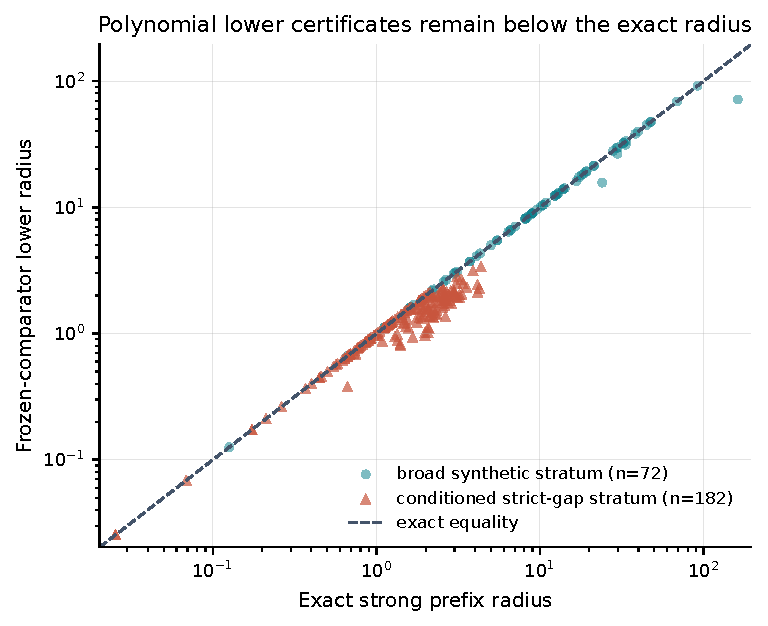
\includegraphics[width=\linewidth]{figures/certificate_brackets.pdf}
\caption{Frozen lower and inverse upper brackets.}
\end{subfigure}\hfill
\begin{subfigure}[t]{0.48\linewidth}
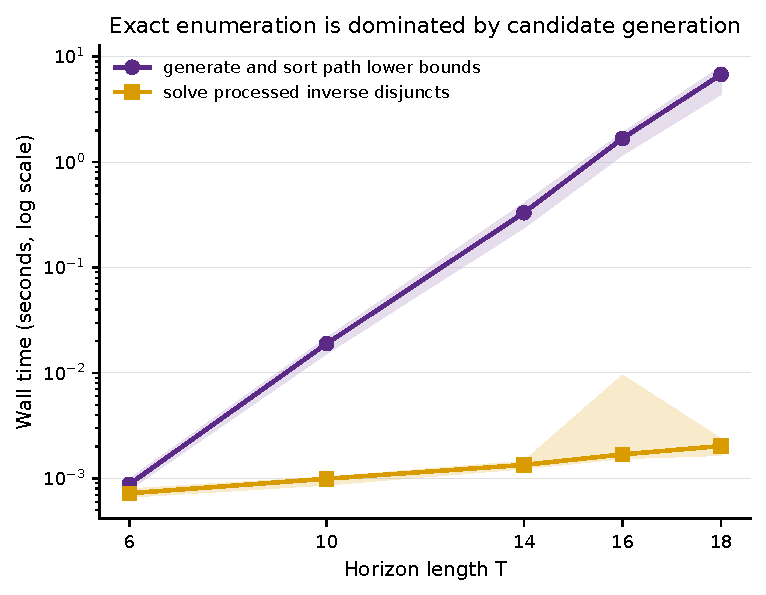
\includegraphics[width=\linewidth]{figures/exact_scaling.pdf}
\caption{Exact enumeration: candidate generation dominates.}
\end{subfigure}

\vspace{1em}
\begin{subfigure}[t]{0.48\linewidth}
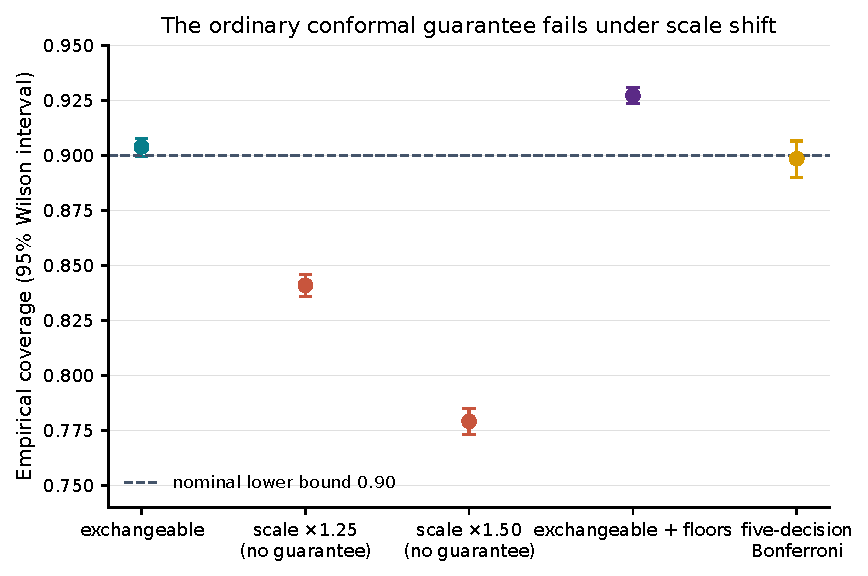
\includegraphics[width=\linewidth]{figures/calibration_coverage.pdf}
\caption{Exchangeable coverage and scale-shift controls.}
\end{subfigure}\hfill
\begin{subfigure}[t]{0.48\linewidth}
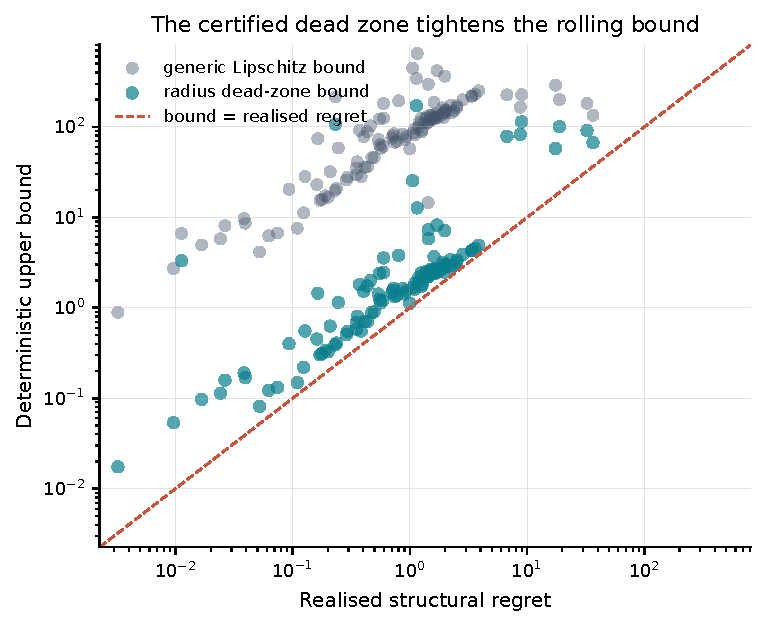
\includegraphics[width=\linewidth]{figures/rolling_bounds.pdf}
\caption{Generic and certified dead-zone bounds.}
\end{subfigure}
\caption{Audit summaries. The colours distinguish evidence strata rather than imply a common probability model.}
\label{fig:audit}
\end{figure}

At $T=18$, the median instance generated 126,976 outside candidates; median bound generation took 12.10 s while the solved disjunct itself took 0.0051 s. Two of the six $T=18$ exact-benchmark cases overran the 15 s wall limit during atomic candidate generation, before solving a disjunct; this leaves 28 of 30 benchmark instances optimal and two explicitly unresolved, with zero solver failures. A recorded hard case with 129,024 paths likewise overran a 5 s exact limit before solving a disjunct. Its polynomial bracket $[4.121,6.128]$ took about 0.005 s, and a MILP probe at $1.01$ times the safe lower bound proved ``no'' in about 0.56 s. \Cref{thm:outsidecount} explains these observations exactly ($126{,}976=2^{17}-2^{12}$ and $129{,}024=2^{17}-2^{11}$), and the stratified evidence below explains the observed practicality boundary.

\subsection*{Corpus equivalence gate and preregistered scaling benchmark}

Before any scaling claim, the compact model of \cref{sec:compact} was
required to reproduce the release's own exact corpora
(\texttt{results/raw/addendum\_equivalence.csv}): the regenerated
exact-certification instances ($T\le8$, all protected depths) and the
exact-benchmark instances ($T\le18$). The 627 rows fall into five disjoint evidence classes. There are 305
\texttt{exact\_match\_certified} compact-model comparisons, each with an
exactly re-verified witness; 247 \texttt{exact\_rational\_equality}
comparisons between direct and decomposed certified enumeration. A further 55
benchmark-search rows form a platform-sensitive partition: the frozen macOS
replay produced 27 \texttt{float\_match\_certified} comparisons whose numerical
search result is paired with an exact witness check, and 28
\texttt{reference\_unresolved} rows, compared with 30 and 25 respectively in
the preliminary Linux replay. The remaining 20 rows are
\texttt{unresolved\_pair}. There were zero disagreements within the relation
warranted by each class. The 48 unresolved rows remain part of the denominator
and are not exact validations.
The gate also exposed one defect in an early witness-repair path (a floating
witness inflated by $1+2^{-12}$ before certification); certification now
derives the exact binding-comparator tie instead.

The scaling benchmark was then run under a design frozen and hashed
before execution (\path{docs/benchmark_preregistration_addendum.md}):
$T\in\{18,25,35,50,75,100\}$, families regular, near-tie and adversarial
(floor-heavy and strict-gap), two replicates, protected depth
$k=\lceil m/2\rceil$ plus a full-path contrast at $T=18$; per-solve caps
of 60 s (180 s for enumeration) and a candidate-guard threshold of
$2^{21}$; 210 recorded solves, no cap or grid deviations during the run
(one post-run summary recomputation from unchanged raw rows is recorded
in the summary's deviation list). The preregistered outcomes:

\begin{itemize}
\item \textbf{P1 (largest resolved horizon).} Exhaustive enumeration
resolved nothing beyond $T=18$: all 30 attempts at $T\ge25$ were refused
by the closed-form candidate guard ($N_{\mathrm{out}}>2^{21}$, disclosed
before generation, not a timeout). The arc-product decision model, both
compact models and the polynomial bracket all reached $T=100$; the
compact minimum-radius model solved 36 of 42 instances to optimality
(median 0.13 s at $T=18$, 60 s at $T=100$; six time-limit incumbents at
the largest horizons), and every optimum carried an exactly re-verified
witness whose radius respected the certified frozen lower bound in all
42 cases.
\item \textbf{P2 (decision wall time).} On the 42 common probes the
compact decision model was faster than the released arc-product model in
every cell, with a median wall-time ratio of $28.7\times$ (interquartile
$16.4\times$--$76.9\times$); it solved all 42 probes to optimality
(median branch-and-bound node counts between 1 and 80), while the
arc-product model hit its cap 13 times.
\item \textbf{P3 (bracket width).} The polynomial certificate alone
closed exactly in 32 of 42 cells (median relative width 0; maximum
0.646), at median 3.0 s even at $T=100$ in exact rational arithmetic.
\end{itemize}

The practical conclusion matches \cref{cor:enumexp}: the polynomial
bracket plus the compact exact model is the deployable escalation path,
and exhaustive enumeration is not an ordinary-horizon method --- its
refusals are now principled disclosures of a closed-form count rather
than timeouts.

The tests were produced in the same workflow as the code. They increase internal confidence but do not constitute independent reproduction.

\section{Illustrative real-demand case}\label{sec:case}

The UCI \emph{Daily Demand Forecasting Orders} dataset contains 60 daily observations from a Brazilian logistics company, 12 predictors and a total-orders target, with no missing cells \parencite{UCIDailyDemand2016}. The local CSV has SHA-256
\begin{center}
\texttt{adf8dda021beae76b13b1cbb5b3c075d064f03b3353a711c1ddc357c6f89e924}.
\end{center}
The exact public-mirror URL used to obtain the local bytes was not preserved. The release therefore records a chain-of-custody gap, checks the file against the official UCI schema and hash-locks the analysed bytes. A clean reproduction should obtain the file from the official UCI archive, record its hash, and resolve any difference from the locked bytes before analysis.

This is \emph{not} a field validation. Observed demand is real; forecast vintages and costs are reconstructed. A causal pooled direct ridge model creates 31 overlapping eight-day windows. The old forecast uses information through three days before the first target, the new forecast through two days before it. Only target lags, rolling target means and known target-calendar variables enter; contemporaneous future predictors from the source table are excluded. Eight windows estimate one pooled norm scale, 11 calibrate a split-conformal threshold at $\alpha=0.20$, and 12 remain for retrospective policy evaluation. Reusing one threshold across all 12 evaluation windows has no simultaneous coverage guarantee.

Setup costs $\{\pounds60,\pounds120,\pounds240\}$ and daily holding costs $\{\pounds0.06,\pounds0.12,\pounds0.24\}$ per order are stylised: monetary symbols denote \emph{stylised cost units parameterised in pounds}, not an empirical calibration of the organisation's economics. The primary design uses $K=\pounds120$ and $h=\pounds0.12$. The decision outcome is structural regret under realised demand in those stylised units, not the original organisation's financial loss. The 12 evaluation windows \emph{overlap} and are not independent replicates; totals over them describe this one reconstruction only.

\begin{table}[t]
\centering
\caption{Primary illustrative policy comparison over 12 reconstructed, overlapping evaluation windows. Regret is in stylised cost units parameterised in pounds.}
\label{tab:case}
\small
\begin{tabularx}{\linewidth}{@{}XrrX@{}}
\toprule
Policy & Mean periods committed & Total structural regret (stylised) & Boundary record \\
\midrule
Polynomial certificate only & 0.17 & \pounds0.00 & One unresolved boundary. \\
Certificate plus exact escalation & 0.33 & \pounds0.00 & One escalation; no unresolved boundary. \\
Old-plan one cycle / fixed 2-period fence & 2.08 & \pounds114.80 & Revision retained the commitment in 10 of 12 windows. \\
Fixed 3-period fence & 3.92 & \pounds308.22 & Revision retained the commitment in 10 of 12 windows. \\
Fixed 4-period fence & 4.17 & \pounds308.22 & Regret coincides with the 3-period fence here: the additional committed period matched the unrestricted benchmark in every window. \\
Updated-plan one cycle & 2.25 & \pounds73.33 & Formed after the later reconstructed vintage. \\
Unrestricted realised-demand benchmark & 0 & \pounds0.00 & Clairvoyant and not implementable. \\
\bottomrule
\end{tabularx}
\end{table}

\begin{figure}[t]
\centering
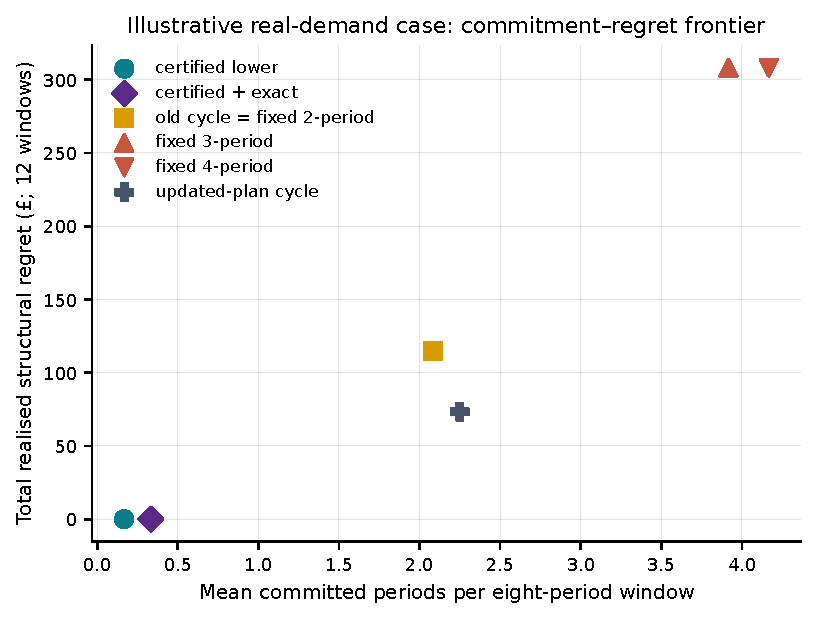
\includegraphics[width=0.82\linewidth]{figures/uci_policy_frontier.pdf}
\caption{Illustrative commitment--regret frontier under the primary stylised cost design. Twelve windows are too few to support a comparative effectiveness claim.}
\label{fig:case}
\end{figure}

The case demonstrates four points. The software can ingest forecast vintages and return safe, unsafe or unresolved boundaries. The lower certificate may be too conservative to commit much. Exact escalation can close a material boundary. Fixed fences trade more commitment for structural regret in this particular reconstruction. The sample, overlap, reconstructed vintages and stylised costs prevent generalisation.

\section{Bounded decision protocol}\label{sec:protocol}

The system returns a decision record, not a blanket instruction to commit.

\begin{enumerate}[label=\textbf{Step \arabic*.},leftmargin=5.2em,itemsep=0.45em]
\item \textbf{Freeze the object.} Record $K,q,\dhat,\ellv,w$, units, forecast vintage, input hash and model exclusions. Verify ordered slopes.
\item \textbf{Audit nominal degeneracy.} Construct the optimal-arc graph, report the longest common optimal prefix and use a deterministic tie-break for any complete comparator.
\item \textbf{Compute the certified bracket.} Retain the exact-rational lower radius, exposed outside path, exact tie witness, any certified upper witness, the infinity status (no outside path, saturation, or not infinite) and search metadata for each $k$. Archive the decision record together with its independent-checker verification.
\item \textbf{Calibrate once for the stated decision.} Align revision rows by product class, horizon, vintage and information set; audit missingness and drift; freeze weights before scoring. For repeated prespecified decisions, allocate error explicitly.
\item \textbf{Apply three-way triage.} Commit only when the calibrated threshold is strictly below the certified lower radius. A threshold at or above a certified upper radius has an exactly verified destabilising witness. The interval between them is unresolved.
\item \textbf{Escalate selectively.} Run the exact disjunction or fixed-radius MILP only when resolving the interval has enough decision value. Preserve all timeouts, gaps and lower/upper bounds. Never recode unresolved as safe.
\item \textbf{Monitor realised structural loss.} Replan at disclosed cycle boundaries, maintain the information structure and quantity-recourse assumptions, and compare realised residuals with \eqref{eq:rollingbound}.
\item \textbf{Govern model exceptions.} Capacity, minimum quantities, joint setups, supplier locks, service levels and manual overrides lie outside this certificate unless represented in the optimisation model.
\end{enumerate}

\begin{table}[htbp]
\centering
\caption{Outputs and their bounded meanings.}
\label{tab:outputs}
\begin{tabularx}{\linewidth}{@{}p{0.22\linewidth}p{0.32\linewidth}X@{}}
\toprule
Output & Warranted statement & Unwarranted inference \\
\midrule
Certified $\rholo$ & Every admissible revision strictly inside it retains the prefix; computed in exact arithmetic & It need not equal the exact strong radius. \\
Certified $\rhohi$ & An exactly verified destabilising witness exists at that radius & It does not prove no closer outside path exists. \\
Proven infinity & Either no outside path exists, or a certified positive residual gap survives maximal admissible reduction & Solver-presumed infinities are never published as proven. \\
Closed bracket / exact result & Nearest structural prefix change under the stated model & It is not a forecast probability. \\
Conformal threshold & One-step marginal revision coverage under exchangeable scores & It is not conditional or time-uniform under drift. \\
Rolling bound & Worst-case structural regret with quantity recourse & It is not expected financial loss or service impact. \\
Illustrative case & End-to-end feasibility on real observed demand with reconstructed inputs & It is not field validation. \\
\bottomrule
\end{tabularx}
\end{table}

\section{Glossary and computational status vocabulary}\label{sec:glossary}

\begin{table}[htbp]
\centering
\caption{Terms used in the theorem statements, software records and audit files.}
\label{tab:glossary}
\small
\begin{tabularx}{\linewidth}{@{}p{0.27\linewidth}X@{}}
\toprule
Term or status & Meaning \\
\midrule
Forced-source graph & The declared path model in which every complete path starts at period 1 and path nodes remain distinct even when an empty zero-cost setup separates them. \\
Classical active horizon & The ordinary uncapacitated lot-sizing interpretation under $\ell_1>0$ and $K_i>0$ for $i\ge2$, as transferred by \cref{thm:semanticbridge}. \\
Inside envelope $A_k$ & Minimum cost over all continuations that retain the protected node prefix. Its optimiser may change with demand. \\
Outside envelope $B_k$ & Minimum cost over paths that leave the protected prefix at or before its end. \\
Strong radius $\rho_{k,w}$ & Distance to the nearest admissible demand at which an outside optimum ties or beats the inside envelope. \\
Frozen radius $\rhofr_{k,w}$ & Polynomial lower certificate obtained by comparing every outside path with one fixed nominal complete path. \\
Single-detour edge witness & A co-optimal inside/outside adjacent path pair that differs only between one divergence and one remergence node. \\
\texttt{exact\_certified} & Candidate enumeration and exact verification close the strong radius to one rational value. \\
\texttt{certified\_interval} & Exact lower and feasible upper witnesses are valid, but the nearest value is not closed. \\
\path{enumeration_completed_with_certified_interval} & All permitted candidates were processed, but at least one disjunct remains unresolved; completion of enumeration is not exact certification. \\
\path{refused_by_candidate_guard} & The closed-form candidate count exceeded the predeclared cap; no safety conclusion follows. \\
\path{solver_level_only} & A mixed-integer search result lacks the exact witness or closing bound needed for a certified classification. \\
\bottomrule
\end{tabularx}
\end{table}

\section{Scope, failure modes and research frontier}\label{sec:scope}

\paragraph{Model scope.}
The theory covers one uncapacitated item, deterministic demand conditional on a scenario, linear costs, no backlogging and ordered reduced slopes. Capacity, joint setups, minimum order quantities, perishability, substitution and service constraints change the feasible family and may destroy the formulas.

\paragraph{Demand domain and semantic mode.}
The admissible set has coordinate floors and no extra upper bounds beyond the radius box. Forced-source graph mode permits zero first-period demand and costless empty setup nodes because those are explicit graph decisions. Classical active-horizon mode requires $\ell_1>0$ and $K_i>0$ for $i\ge2$; only under those conditions does \cref{thm:semanticbridge} transfer setup-prefix conclusions to the ordinary lot-sizing model. Directionally asymmetric norms require new pairwise and breakpoint derivations.

\paragraph{Nominal choice.}
The exact radius is a property of a node prefix. The frozen certificate is conditional on the selected complete nominal comparator. The release makes this dependency visible and recommends protecting only the common nominal prefix unless a disclosed secondary criterion selects among optima.

\paragraph{Numerical assurance.}
Every certified value is computed or a posteriori verified in exact rational arithmetic, decision records carry machine-checkable witnesses, and an independent checker re-verifies them; the previous version's tolerance-based safe margins are gone. The remaining assurance gaps are stated exactly: for $T>12$ the checker re-verifies achievability, infinity and consistency but relies on the package's internally cross-checked parametric computation for lower-bound minimality; mixed-integer ``no'' decisions remain solver-level evidence unless the certified bracket already covers them; and neither implementation has proof-assistant verification. The exact layer decides the rational instance actually supplied: plain JSON numbers are read as their exact binary values, and users whose data are decimal should supply numeric strings, which are parsed as exact decimals.

\paragraph{Statistical scope.}
Exchangeability can fail under forecast-system changes, promotions, censoring, missing horizons or distribution shift. The negative controls show the direction of risk, not a universal correction. A sequential version should state its target, filtration and long-run or finite-horizon guarantee explicitly.

\paragraph{External validity.}
The synthetic audit tests correctness and boundary cases. The UCI case uses real demand but synthetic vintages and costs. A field study should preserve actual forecast vintages, release decisions, order quantities, capacity constraints, service outcomes and expediting costs, and compare against fixed fences and unrestricted replanning.

\paragraph{Open exact complexity.}
Generic partial inverse and partial anti-inverse shortest paths are already hard: NP-complete on DAGs even for one required arc with increase-only weights \parencite{LeyMerkert2025} and strongly NP-hard under $L_1$ and $L_\infty$ for forbidden elements \parencite{Gassner2009}. The present analysis sharpens the boundary on both sides. Algorithmically, the released escalation is now proved worst-case exponential --- it materialises $2^{T-1}-2^{\max\{T-v_k,0\}}$ outside candidates before its first inverse programme (\cref{thm:outsidecount,cor:enumexp}) --- while the decision problem itself lies in NP with polynomial-bit witnesses (\cref{prop:np}); an exponential implementation must not be mistaken for problem hardness (\cref{rem:algnotproblem}). Structurally, the prefix radius decomposes exactly into at most $k$ one-protected-arc radii (\cref{cor:arcreduction}), so the open question is now confined to its narrowest core: can a rational demand vector in the weighted floor-truncated box make one specified Wagner--Whitin outgoing arc cease to be uniquely optimal, under correlated costs $K_i+q_i(D_j-D_i)$ and ordered slopes? Neither a polynomial algorithm nor a hardness reduction preserving the demand-induced cost map is known. The compact production-balance model (\cref{thm:compact}) supplies a polynomial-size exact formulation --- solver work remains NP-type --- and its linear relaxation is the natural place to search for integrality or a fractional counterexample seeding a reduction.

\paragraph{Novelty status.}
A page-specific reading of the supplied Richter--V{\"o}r{\"o}s (1989) scan closes the source-specific question that motivated the acquisition: that paper studies scalar-parametric stability of one fixed regeneration-point solution and does not state the protected-prefix, moving-continuation or weighted demand-ball object developed here (\cref{sec:literature}). The release records the inspected pages and the hash of the supplied Pages bundle. This is strong negative evidence against a collision in the closest identified source. It is not an exhaustive priority proof: the search is targeted, adjacent same-programme papers remain less completely inspected, and independent bibliographic attestation remains a later assurance target.

\section{Conclusion}

The decision object is the weighted distance from the current demand forecast to the nearest instance on which an optimal Wagner--Whitin path may leave a protected replenishment prefix. Reduced arcs $K_i+q_i(D_j-D_i)$ make this geometry tractable in layers.

A fixed outside path has an exact floor-aware tie radius. A formally specified prefix-deviation graph and a repaired Charnes--Cooper argument compute the frozen-comparator radius in polynomial time; the released implementation computes the same value in exact rational arithmetic through breakpoint binary search and finitely terminating parametric shortest paths, and ships every certificate with independently checkable witnesses. That value is a valid lower certificate, exact for a full path and sometimes strict for a partial prefix. A compact fixed-path inverse programme turns the exposed competitor into a feasible upper bound; a closing witness or coincident bounds can certify the exact strong radius without enumeration. The finite disjunction and mixed-integer model remain exact escalation mechanisms, but their practical scale is unresolved.

The escalation layer is now characterised without conflating algorithmic cost with problem complexity. The released disjunction is worst-case exponential by an explicit candidate count known before generation, and the implementation can refuse it before front-loading that work. The decision problem lies in NP under rational encoding; the strong radius is the minimum of at most $k$ one-arc suffix radii; and every finite boundary has an optimal-face edge witness formed by one structural detour. A compact production-balance model gives a polynomial-size exact formulation, although solving it remains mixed-integer work. The exact complexity of the demand-induced one-arc problem remains open, and the paper states that frontier rather than inferring hardness from an exponential routine.

Nominal-degeneracy analysis prevents arbitrary solver ties from masquerading as commitment robustness. One-step conformal calibration gives a marginal probability statement only under exchangeability and domain alignment. The rolling theorem prices structural setup decisions with quantity recourse and supplies a deterministic dead zone. Producer-side tests and an illustrative real-demand case support implementation plausibility while leaving independent reproduction and field validity open.

The resulting contribution is a bounded decision architecture with two explicit semantic layers. Its graph theorems apply to the forced-source model; its classical setup-schedule interpretation applies only through the active-horizon bridge. Certified outputs are rational and witness-backed, and the interface distinguishes certified-safe, witnessed-unsafe, certified-interval, refused and solver-level states. The source-specific Richter--V{\"o}r{\"o}s reading supports the contribution boundary while leaving exhaustive priority open. Capacity, multi-item coupling, service outcomes and live forecast processes remain outside the warranted claim and require new theory or field evidence.

\clearpage
\appendix

\section{Proof details and edge cases for the polynomial certificate}\label{app:proof}

For an outside path $Q$, write $c_{Q,t}=\beta_{Q,t}-\beta_{P^\star,t}$. Its worst frozen gap at radius $r$ is
\[
F_Q(r)=\kappa_Q-\kappa_{P^\star}
+\sum_{c_{Q,t}<0}c_{Q,t}(\dhat_t+r/w_t)
+\sum_{c_{Q,t}>0}c_{Q,t}\max\{\ellv_t,\dhat_t-r/w_t\}.
\]
The expanded graph adds the same setup cost and coefficient contribution once for every physical arc, so \eqref{eq:aintercept}--\eqref{eq:intervalgap} reproduce $F_Q$ exactly.

If distinct breakpoints coincide numerically, the implementation collapses them before forming intervals. A coordinate with $\dhat_t=\ellv_t$ is saturated at radius zero. Both neighbouring formulae agree at a finite endpoint, so assigning a tie to the first interval does not change the earliest crossing. If $(b^\ell)^\top x=0$, then $F_x$ is constant on the interval and cannot cross after a safe left endpoint. If every path has zero denominator on the final interval, all remaining positive differences are floor-saturated and no negative difference is available to reduce a gap; the radius is infinite.

The linear programme can return a convex combination when several paths share the same ratio. Since a linear objective attains its optimum at an extreme point, one may recover a path by resolving with an infinitesimal deterministic arc-order tie-break or by running a shortest path at the returned boundary. Substitution into \eqref{eq:worstrevision} gives a directly checkable half-space witness. The implementation checks that the recovered path's pairwise radius lies in the active interval; otherwise it reports that numerical witness recovery failed rather than silently certifying a path.

\section{Exact destabilising set as a union of polyhedra}

For each $Q\in\cO_k$, define
\[
\mathcal D_Q=\{d\ge\ellv:C_Q(d)\le C_P(d)\text{ for every }P\in\cI_k\}.
\]
Then
\[
\mathcal D_k=\bigcup_{Q\in\cO_k}\mathcal D_Q,
\qquad
\rho_{k,w}=\operatorname{dist}_{\infty,w}(\dhat,\mathcal D_k).
\]
Each $\mathcal D_Q$ is a polyhedron. It has an exponential direct description with one inequality per inside path and the compact extended description in \eqref{eq:fixedlp}. The frozen certificate replaces $\mathcal D_Q$ by the larger half-space $\{d:C_Q(d)\le C_{P^\star}(d)\}$, explaining both safety and possible conservatism.

\section{Computational design, exclusions and missingness}\label{app:compute}

\begin{longtable}{@{}p{0.22\linewidth}p{0.72\linewidth}@{}}
\caption{Frozen computational design.}\label{tab:design}\\
\toprule
Component & Design and missingness treatment \\
\midrule
\endfirsthead
\toprule
Component & Design and missingness treatment \\
\midrule
\endhead
Certificate audit & 258 generated instances: 162 broad synthetic and 96 conditioned adversarial. Every generated instance appears in the raw manifest. The conditioned set targets strictness and is excluded from prevalence interpretation. Partial prefixes and full paths are both tested. \\
Graph audit & Exhaustive path-set comparison for 62 small expanded graphs. No missing or failed graph cases. \\
Fixed competitor & 96 compact LPs compared with separately constructed explicit inside-path LPs. No solver failures. \\
Exact benchmark & 30 instances across five horizons, three regimes and two replicates per cell. Exact limit 15 s includes candidate generation. Twenty-eight were optimal; two $T=18$ cases timed out during atomic candidate generation before processing a disjunct. No solver failure occurred. \\
MILP benchmark & 24 fixed-radius probes with 2 s limits. Two returned feasible incumbents without closing bounds and remain unresolved; they are not counted as correct negative or positive decisions. \\
Calibration & Trial counts, calibration sizes, ranks, covered counts and Wilson intervals appear in raw and processed files. Scale-shift rows are negative controls to which the exchangeability theorem does not apply. Inadmissible floor revisions receive infinite scores rather than being dropped. \\
Rolling & 240 broad cases, 120 strict-gap conditioned cases, 100 exact-witness destabilising cases and two edge cases. All realised vectors satisfy floors. Frequencies in conditioned strata are not prevalence estimates. \\
UCI data & 60 rows, 13 columns and zero missing cells in the analysed CSV. The exact local mirror URL is missing from provenance; official UCI metadata, schema, licence and DOI are recorded, and the bytes are hash-locked. Forecast vintages and costs are reconstructed and clearly separated from observed demand. \\
Software & Python 3.12.11, NumPy 2.3.5, SciPy 1.17.0 with embedded HiGHS 1.8.0 (MIT), pandas 2.2.3 and Matplotlib 3.10.8 in the frozen macOS run. HiGHS proposes LP/MIP search results but has no certification role. The release includes a lockfile, one-command verifier and deterministic seed. A producer-created fresh environment replay passed with isolated wheel import; no independent clean-room environment has replayed the package. \\
\bottomrule
\end{longtable}

\section{Notation}

\begin{longtable}{@{}p{0.22\linewidth}p{0.72\linewidth}@{}}
\toprule
Symbol & Meaning \\
\midrule
$T$ & Number of periods. \\
$K_i,p_i,h_i$ & Setup, production/purchase and one-period holding costs. \\
$H_i,q_i$ & Cumulative holding adjustment and ordered reduced slope. \\
$D_j$ & Demand accumulated before node $j$. \\
$P^\star,\pi_k$ & Selected nominal complete path and its first $k$ arcs. \\
$\cI_k,\cO_k$ & Paths retaining and leaving the protected prefix. \\
$A_k,B_k$ & Best inside and outside path-cost envelopes. \\
$w,\ellv$ & Positive norm weights and coordinate demand floor. \\
$\rho_{k,w}$ & Exact strong prefix-stability radius. \\
$\rhofr$ & Frozen-comparator lower radius. \\
$\rholo,\rhohi$ & Polynomial lower and feasible upper bracket. \\
$\kappa_P,\beta_P$ & Constant and demand-coefficient vector of path $P$. \\
$\Gamma_a$ & Exact weighted coefficient diameter of suffix paths. \\
$R_\pi(d)$ & Bellman residual of an executed structural block. \\
$V_i(d)$ & Optimal suffix value from node $i$; $V_{T+1}=0$. \\
$E_r,O_r$ & Protected-arc and best-diverging values at $v_r$ (\cref{sec:decomposition}). \\
$\rho_r$ & One-protected-arc radius at $(v_r,v_{r+1})$. \\
$N(i),\lvert\cO_k\rvert$ & Suffix path count $2^{\max\{T-i,0\}}$ and outside-path count. \\
$y,x,I$ & Setup, production and inventory variables of the compact model. \\
\bottomrule
\end{longtable}

\printbibliography

\end{document}
